%%%%%%%%%%%%%%%%%%%%%%%%%%%%%%%%%%%%%%%%%%%%%%%%%%%%%%%%%%%%%%%%%%%%%%%%%%%%
% AGUJournalTemplate.tex: this template file is for articles formatted with LaTeX
%
% This file includes commands and instructions
% given in the order necessary to produce a final output that will
% satisfy AGU requirements, including customized APA reference formatting.
%
% You may copy this file and give it your
% article name, and enter your text.
%
%
% Step 1: Set the \documentclass
%
%

%% To submit your paper:
\documentclass[draft]{agujournal2019}
\usepackage{url} %this package should fix any errors with URLs in refs.
\usepackage{lineno}
\usepackage[inline]{trackchanges} %for better track changes. finalnew option will compile document with changes incorporated.
\usepackage{soul}
\usepackage{gensymb}
\usepackage{placeins}
\usepackage{multirow}
\usepackage{setspace}

\linenumbers
%\onehalfspacing

\usepackage{todonotes}
%%%%%%%
% As of 2018 we recommend use of the TrackChanges package to mark revisions.
% The trackchanges package adds five new LaTeX commands:
%
%  \note[editor]{The note}
%  \annote[editor]{Text to annotate}{The note}
%  \add[editor]{Text to add}
%  \remove[editor]{Text to remove}
%  \change[editor]{Text to remove}{Text to add}
%
% complete documentation is here: http://trackchanges.sourceforge.net/
%%%%%%%

\draftfalse

%% Enter journal name below.
%% Choose from this list of Journals:
%
% JGR: Atmospheres
% JGR: Biogeosciences
% JGR: Earth Surface
% JGR: Oceans
% JGR: Planets
% JGR: Solid Earth
% JGR: Space Physics
% Global Biogeochemical Cycles
% Geophysical Research Letters
% Paleoceanography and Paleoclimatology
% Radio Science
% Reviews of Geophysics
% Tectonics
% Space Weather
% Water Resources Research
% Geochemistry, Geophysics, Geosystems
% Journal of Advances in Modeling Earth Systems (JAMES)
% Earth's Future
% Earth and Space Science
% Geohealth
%
% ie, \journalname{Water Resources Research}

\journalname{Water Resources Research}


\begin{document}

%% ------------------------------------------------------------------------ %%
%  Title
%
% (A title should be specific, informative, and brief. Use
% abbreviations only if they are defined in the abstract. Titles that
% start with general keywords then specific terms are optimized in
% searches)
%
%% ------------------------------------------------------------------------ %%

% Example: \title{This is a test title}

\title{Automatic input variable selection for analog methods using genetic algorithms}

%% ------------------------------------------------------------------------ %%
%
%  AUTHORS AND AFFILIATIONS
%
%% ------------------------------------------------------------------------ %%

% Authors are individuals who have significantly contributed to the
% research and preparation of the article. Group authors are allowed, if
% each author in the group is separately identified in an appendix.)

% List authors by first name or initial followed by last name and
% separated by commas. Use \affil{} to number affiliations, and
% \thanks{} for author notes.
% Additional author notes should be indicated with \thanks{} (for
% example, for current addresses).

% Example: \authors{A. B. Author\affil{1}\thanks{Current address, Antartica}, B. C. Author\affil{2,3}, and D. E. Author\affil{3,4}\thanks{Also funded by Monsanto.}}


\authors{P. Horton\affil{1}, O. Martius\affil{1}, and S. L. Grimm\affil{2}}

\affiliation{1}{Institute of Geography, Oeschger Centre for Climate Change Research, University of Bern, Bern, Switzerland}
\affiliation{2}{Center for Space and Habitability, University of Bern, Bern, Switzerland}

\correspondingauthor{Pascal Horton}{pascal.horton@alumni.epfl.ch}

%% Keypoints, final entry on title page.

%  List up to three key points (at least one is required)
%  Key Points summarize the main points and conclusions of the article
%  Each must be 100 characters or less with no special characters or punctuation and must be complete sentences

% Example:
% \begin{keypoints}
% \item	List up to three key points (at least one is required)
% \item	Key Points summarize the main points and conclusions of the article
% \item	Each must be 100 characters or less with no special characters or punctuation and must be complete sentences
% \end{keypoints}

\begin{keypoints}
\item enter point 1 here
\item enter point 2 here
\item enter point 3 here
\end{keypoints}

%% ------------------------------------------------------------------------ %%
%
%  ABSTRACT and PLAIN LANGUAGE SUMMARY
%
% A good Abstract will begin with a short description of the problem
% being addressed, briefly describe the new data or analyses, then
% briefly states the main conclusion(s) and how they are supported and
% uncertainties.

% The Plain Language Summary should be written for a broad audience,
% including journalists and the science-interested public, that will not have 
% a background in your field.
%
% A Plain Language Summary is required in GRL, JGR: Planets, JGR: Biogeosciences,
% JGR: Oceans, G-Cubed, Reviews of Geophysics, and JAMES.
% see http://sharingscience.agu.org/creating-plain-language-summary/)
%
%% ------------------------------------------------------------------------ %%

%% \begin{abstract} starts the second page

\begin{abstract}
.........
\end{abstract}

%% ------------------------------------------------------------------------ %%
%
%  TEXT
%
%% ------------------------------------------------------------------------ %%

\section{Introduction}

Analog methods (AMs) are statistical downscaling techniques \cite{Maraun2010} relying on the inherent relationship between meteorological predictors, usually at a synoptic scale, and local weather \cite{Lorenz1956, Lorenz1969}. Archives of predictor and predictand data are exploited to extract similar meteorological situations and to infer the possible consequences. Daily precipitation is often the predictand of interest, either in the context of operational forecasting \cite<e.g.>[]{Hamill2006, Bliefernicht2010, Marty2012, Horton2012, Hamill2015, BenDaoud2016} or more recently in climate change studies \cite<e.g.>[]{Dayon2015, Raynaud2016b} or past climate reconstruction \cite{Caillouet2016}. AMs are also used for other predictands, such as precipitation radar images \cite{Panziera2011, Foresti2015a}, temperature \cite{DelleMonache2013, Caillouet2016, Raynaud2016b}, wind \cite{DelleMonache2013, DelleMonache2011, Vanvyve2015, Alessandrini2015, Junk2015, Junk2015c}, and solar radiation or power production \cite{Alessandrini2015a, Bessa2015, Raynaud2016b}.

AMs usually consist in a stepwise selection of similar situations based on multiple predictors organized in different consecutive levels of analogy, each of which conditioning the subsequent selection. Each predictor is characterized by the selected meteorological variable, its reference hour and vertical level if relevant, the domain on which it is considered, and the analogy criteria (distance measure) used. For each level of analogy, a certain number of analogs are selected.

A semi-automatic sequential procedure \cite{Bontron2004, Radanovics2013, BenDaoud2016} is usually used to optimize the size of the domain and the number of analogs. However, the predictor variables, vertical levels, hours, and analogy criteria are selected manually, which often results in the comparison of numerous combinations and comprehensive assessments of some parameters ranges. Moreover, this calibration procedure being sequential, i.e. the levels of analogy are calibrated consecutively, it does not handle parameters inter-dependencies. Considering these limitations, \citeA{Horton2017a} introduced a global optimization of the AM using genetic algorithms (GAs). Using this approach, an automatic and objective selection of the predictor hours, the vertical levels, the domains, and the number of analogs became possible and improved the prediction skills of the method \cite{Horton2018a}. A weighting between the predictor variables was also introduced. The only parameters that were left for a manual selection were the meteorological variable and the analogy criteria.

The selection of the predictors for precipitation prediction with AMs in Europe has been the focus of multiple studies aiming at improving the prediction skills. Thus, the relevant predictors are likely to be known nowadays and supported by expert knowledge. However, transferring AMs for a region with different climatic conditions, or for another predictand, would involve a reconsideration of the selected meteorological variables. This work aims at testing a fully automatic optimization of all the parameters of the method, including the selection of the meteorological variables and even the analogy criteria, using GAs. To compare with existing and proven AMs, daily precipitation in central Europe, specifically Switzerland, has been chosen as predictand. Also, as it is often the case, the AM was here calibrated in the perfect prognosis framework, using predictors from reanalyses.

The questions we sought to address are: are GAs able to select both the meteorological variables and the analogy criteria? Do these selections make sense in terms of meteorological processes? What are the potential and limits of such approach?

The paper is organized as follows. Section \ref{data} describes the datasets used for predictors and predictands. Section \ref{methods} presents the principles of AMs and the characteristics of the GAs implementation. Section \ref{software} describes the software used as well as the modifications that were necessary. Section \ref{setup} provides the experiment setup details with the selected meteorological variables and analogy criteria. Section \ref{results} presents the results of different analyses, such as the selection of the best predictor variable, the relevance of different AM structures, and the skill of the optimized methods. Finally, section \ref{conclusions} summarizes the main contributions of the work and open perspectives for applications of the developed approach.


\section{Data}
\label{data}

\subsection{Precipitation Data}
\label{precip}

The precipitation data considered is the RhiresD gridded dataset provided by MeteoSwiss. It is a daily aggregation (from 06:00~UTC of day D to 06:00~UTC of day D+1) at a 2~km resolution, available since 1961. It is produced by an interpolation scheme between gauging stations \cite{Frei1998}. The gridded data was here aggregated on catchments of about 200~km$^2$ (Table \ref{catchments}). These catchments were chosen to cover the different climatic regions of Switzerland \cite{Schuepp1980}, as illustrated in Fig.~\ref{map}.


\begin{figure}[hbt]
	\noindent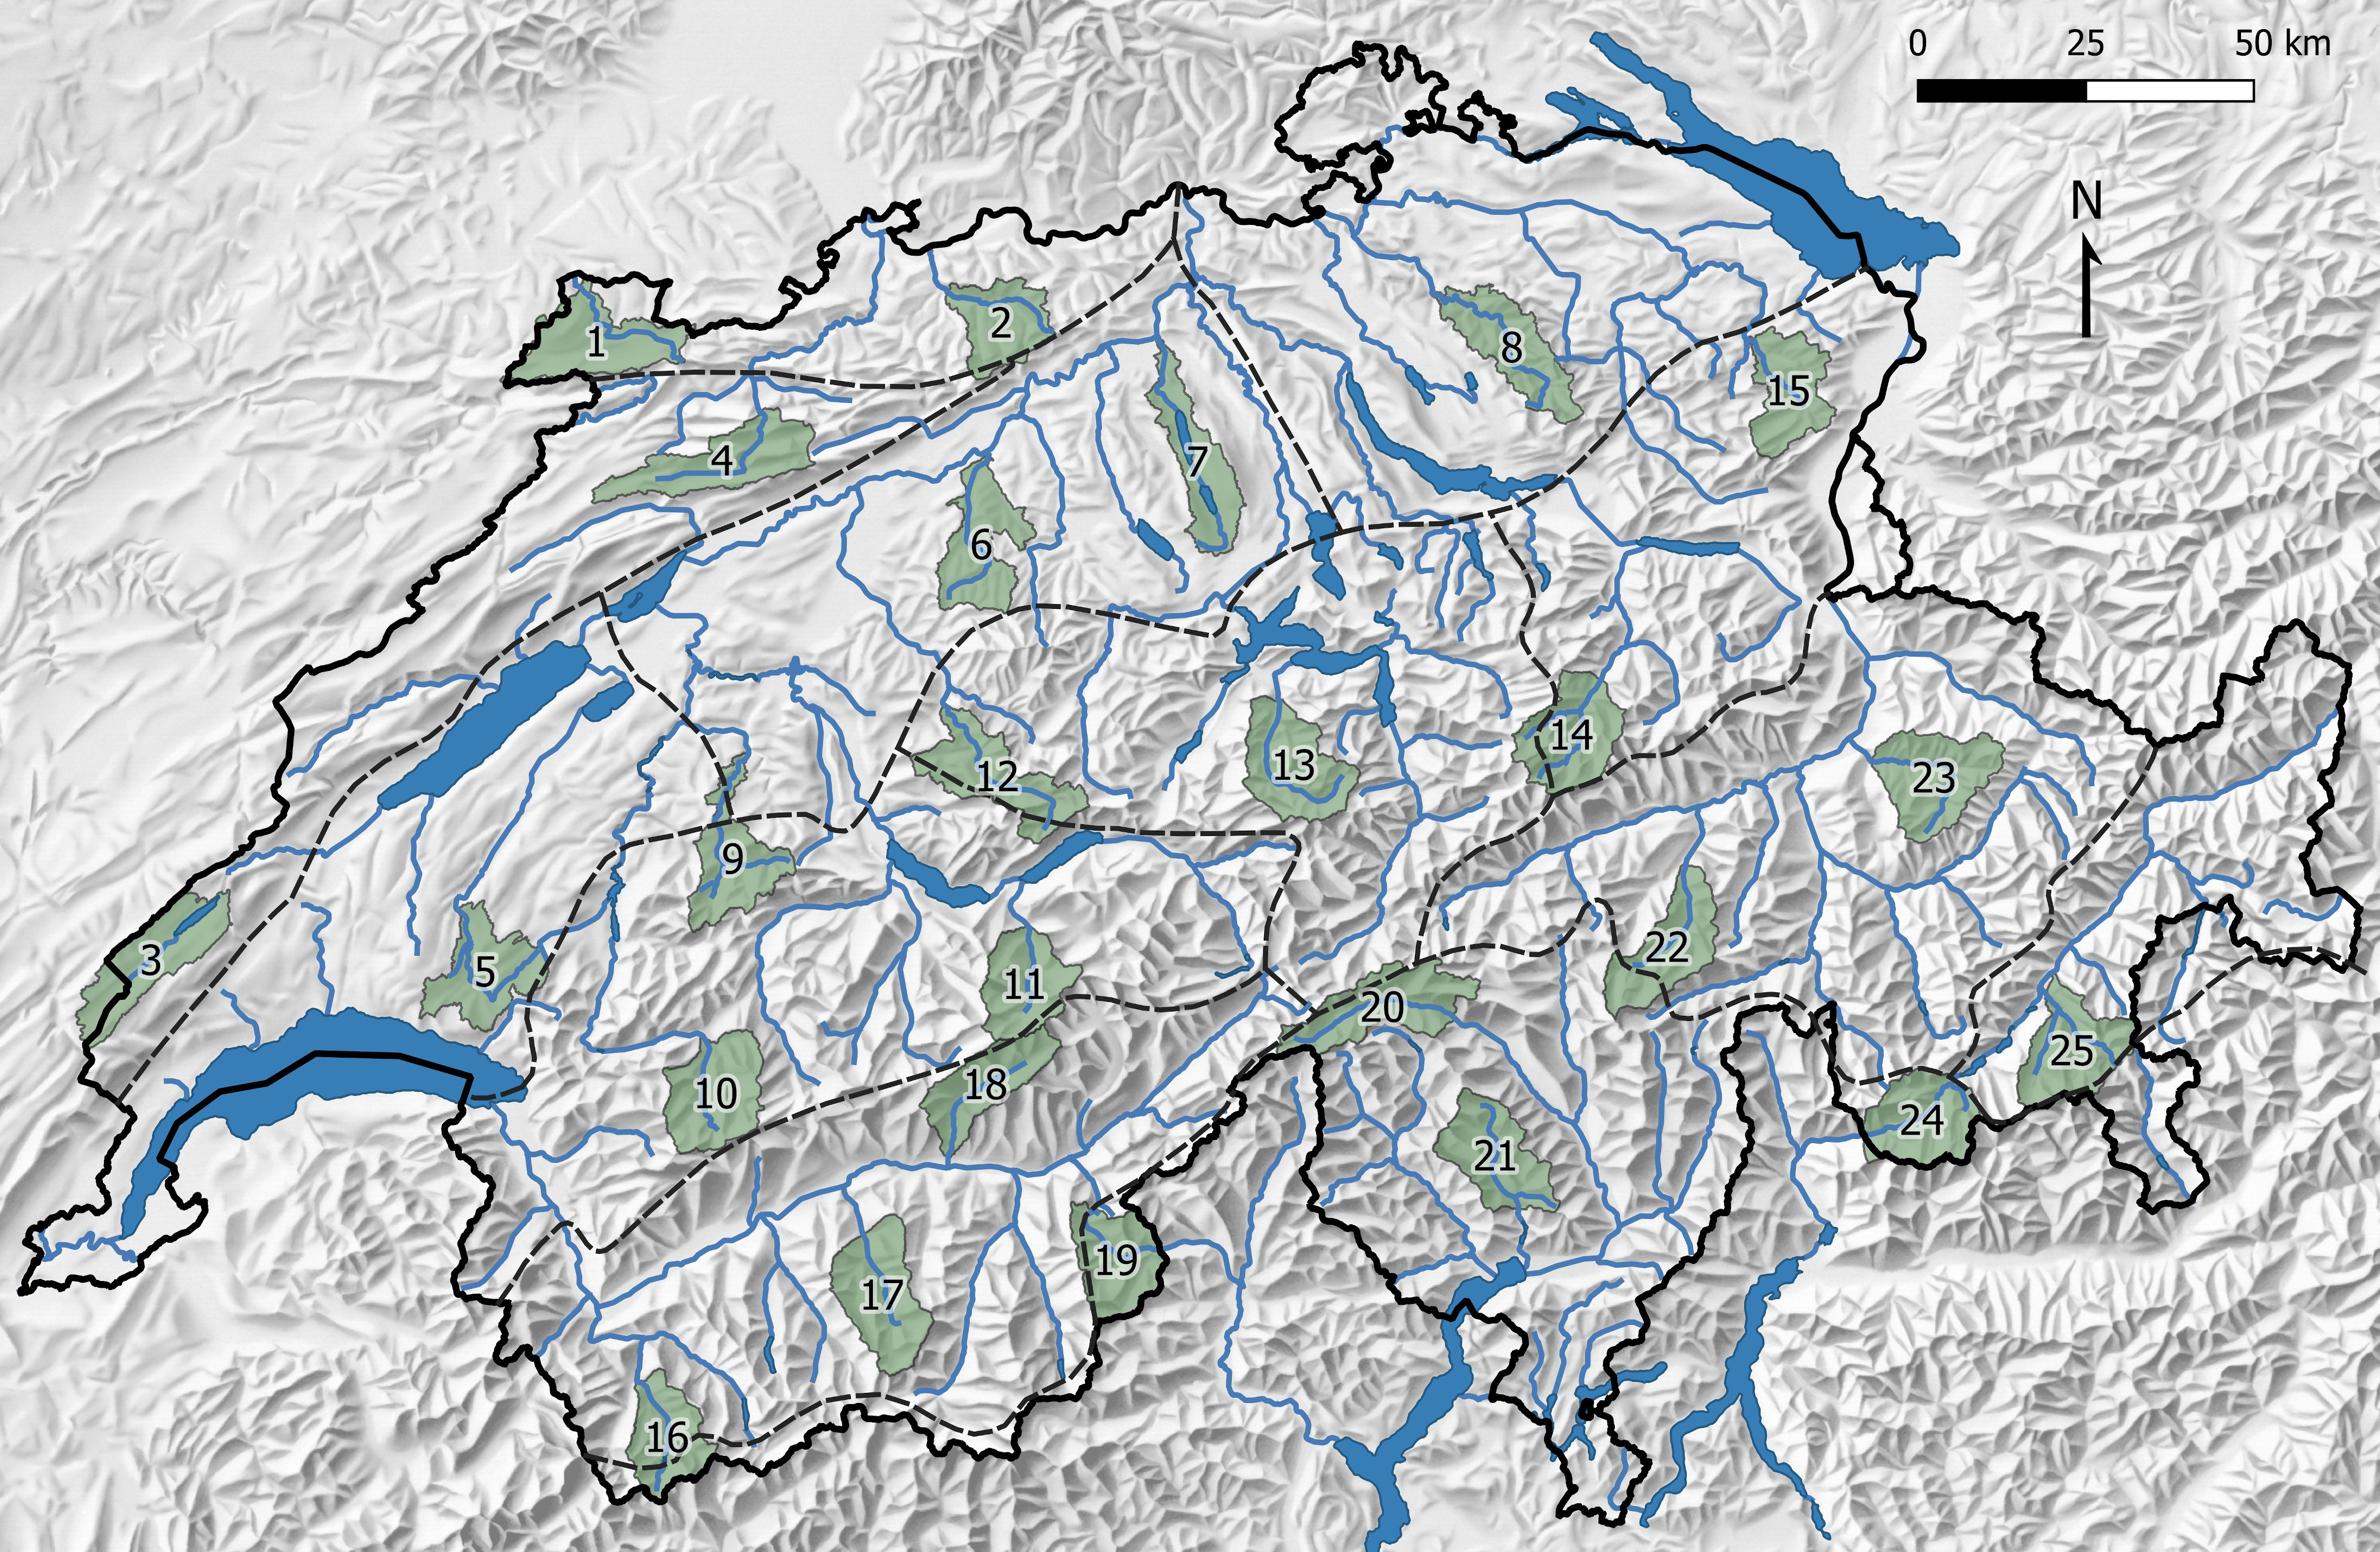
\includegraphics[width=140mm]{figures/map.jpg}
	\caption{Location of the 25 selected catchments in Switzerland along with the climatic regions and the river network (source: SwissTopo, HADES).}
	\label{map}
\end{figure}


\begin{table}[hbt]
	\centering
	\caption{Characteristics of the 25 selected catchments in Switzerland}
	\small
	\setstretch{0.8}
	\begin{tabular}{cllcc}
		\hline 
		Id & Name of the river & Climatic region & Area & Mean elevation \\
		& & & (km$^2$) & (m a.s.l.) \\
		\hline 
		1 & L'Allaine & Eastern Jura & 209.1 & 571 \\
		2 & Ergolz & Eastern Jura & 150.3 & 589 \\
		3 & L'Orbe & Western Jura & 209.3 & 1229 \\
		4 & La Birse & Western Jura & 203.3 & 920 \\
		5 & La Broye & Western Plateau & 184.5 & 791 \\
		6 & Murg & Central Plateau & 184.8 & 658 \\
		7 & Aabach & Central Plateau & 180.0 & 562 \\
		8 & T\"oss & Northeastern part of the Plateau & 189.3 & 745 \\
		9 & Sense & Western part of the Alps northern side & 179.6 & 1238 \\
		10 & La Sarine & Western part of the Alps northern side & 200.8 & 1779 \\
		11 & Weisse L\"utschine & Western part of the Alps northern side & 165.0 & 2149 \\
		12 & Emme & Centrale part of the Alps northern side & 206.9 & 1151 \\
		13 & Engelberger Aa & Centrale part of the Alps northern side & 204.3 & 1654 \\
		14 & Linth & Eastern part of the Alps northern side & 195.7 & 1959 \\
		15 & Sitter & Eastern part of the Alps northern side & 162.2 & 1069 \\
		16 & Dranse d'Entremont & Wallis & 154.2 & 2340 \\
		17 & La Navisence & Wallis & 210.5 & 2541 \\
		18 & Lonza & Wallis & 161.7 & 2370 \\
		19 & Doveria & Southern Alps & 170.5 & 2241 \\
		20 & Ticino & Southern Alps & 208.5 & 2019 \\
		21 & Verzasca & Southern Alps & 187.4 & 1656 \\
		22 & Valser Rhein & North and Central Graubünden & 185.8 & 2215 \\
		23 & Plessur & North and Central Graubünden & 207.7 & 1928 \\
		24 & Mera & Southern Alps & 190.6 & 2142 \\
		25 & Flaz & Engadine & 193.1 & 2599 \\
		\hline 
	\end{tabular} 
	\label{catchments}
\end{table}


\subsection{Reanalysis Datasets}
\label{reanalyses}

This work takes place in the context of the perfect prognosis framework, where the predictors are considered relatively close to the actual states of the atmosphere. As often done in this context, we used variables provided by global reanalyses. These are produced using a single version of a data assimilation system coupled with a forecast model constrained to follow observations. However, homogeneity in time is a challenge due to significant changes in observing systems. Because of these discontinuities in the available observations, some variables from the reanalyses, such as precipitation and evaporation are to be used with great caution \cite{Kobayashi2015}. Moreover, even though most reanalyses provide good quality data over Europe, differences still exist and the choice of the reanalysis dataset can lead to differences in the skill score of the AM that can be larger than the choice of the predictor variables \cite{Horton2018b}. Thus, it was considered advisable to test some of the following analyses with another reanalysis to assess the robustness of the selected variables.

The main reanalysis used in this work is ERA-Interim \cite<ERA-I,>{Dee2011a}, which is produced by the European Centre for Medium-Range Weather Forecasts (ECMWF) and covers the period from 1979 onward. The forecast model uses a hybrid sigma-pressure vertical coordinate on 60 layers and has a T255 horizontal resolution (about 79~km) and a 30~min time step. The output variables have a spatial resolution of 0.75\degree. The present work started before the release of ERA5, the successor of ERA-I.

The Climate Forecast System Reanalysis \cite<CFSR,>{Saha2010a}, provided by NCEP, was also used for the first analysis, which consisted in the selection of the single best predictor for each catchment. The model used to produce CFSR has a horizontal resolution of T382 (about 38~km) and 64 levels on sigma-pressure hybrid vertical coordinates. The period covered is from 1979 onward and the output variables have a spatial resolution of 0.5\degree.

Finally, ERA5 \cite{Hersbach2019} was finally used for the last analysis as it provides more variables and a higher spatial (0.25\degree) and temporal resolution (hourly, but considered here at a 3-hrly time step). ERA5 assimilates significantly more data than ERA-I, and provides, among others, more consistent sea surface temperature and sea ice, an improved representation of tropical cyclones, a better balance of evaporation and precipitation, and improved soil moisture. ERA5 also relies on more appropriate radiative forcing and boundary conditions (e.g., changes in greenhouse gases, aerosols, SST, and sea ice).


\section{Methods}
\label{methods}

\subsection{Analog Methods}
\label{ams}

AMs are based on the rationale that two similar synoptic situations may produce similar local effects \cite{Lorenz1956, Lorenz1969}. It thus consists in extracting similar past atmospheric situations to a target date, as defined by selected predictors, to build a conditional distribution of the predictand of interest, which is often daily precipitation. The analogy is defined by:

\begin{itemize}		
	\item The meteorological variables (predictors).
	\item The vertical levels at which the predictors are selected.
	\item The spatial windows (domains) over which the predictors are compared.
	\item The hours of the day at which the predictors are considered.
	\item The analogy criteria used to rank candidate situations according to their degree of similarity with the target situation.
	\item Possible weights between the predictors.
	\item The number of analog situations $N_{i}$ to retain for the analogy level $i$.
\end{itemize}

AMs usually start with a seasonal preselection to cope with seasonal effects \cite{Lorenz1969}. It is often implemented as a moving window of 120~days centred around the target date \cite{Bontron2004, Marty2012, Horton2012, BenDaoud2016}. Alternatively, the candidate dates can be selected based on similar air temperature at the nearest grid point \cite{BenDaoud2016}. In this work, we used the temporal moving window to reduce the number of potential candidate dates, and thus the processing time.


\begin{table}[hbt]
	\caption{Analog methods considered as references, listed by increasing complexity. The analogy criterion is S1 for Z and RMSE for the other variables.}
	\small
	\setstretch{0.8}
	\begin{tabular}{llllll}
		\hline
		\textbf{Method} & \textbf{P0} & \textbf{L1} & \textbf{L2} & \textbf{L3} & \textbf{Reference} \\ 
		\hline 
		\multirow{2}{*}{\textbf{2Z}} & \multirow{2}{*}{PC} & Z1000@12h &&& \multirow{2}{*}{\citeA{Bontron2004}} \\
		&& Z500@24h &&& \\
		\hline 
		\multirow{4}{*}{\textbf{4Z}} & \multirow{4}{*}{PC} & Z1000@06h &&& \multirow{4}{*}{\citeA{Horton2018a}} \\
		&& Z1000@30h &&& \\
		&& Z700@24h &&& \\
		&& Z500@12h &&& \\
		\hline 
		\multirow{2}{*}{\textbf{2Z-2MI}} & \multirow{2}{*}{PC} & Z1000@12h & \multirow{2}{*}{MI850@12+24h} && \multirow{2}{*}{\citeA{Bontron2004}} \\
		&& Z500@24h &&& \\
		\hline 
		\multirow{4}{*}{\textbf{4Z-2MI}} & \multirow{4}{*}{PC} & Z1000@30h &&& \multirow{4}{*}{\citeA{Horton2018a}}\\
		&& Z850@12h & MI700@24h && \\
		&& Z700@24h & MI600@12h && \\
		&& Z400@12h &&& \\
		\hline 
		\multirow{2}{*}{\textbf{PT-2Z-4MI}} & T925@36h & Z1000@12h & MI925@12+24h && \multirow{2}{*}{\citeA{BenDaoud2016}} \\
		& T600@12h & Z500@24h & MI700@12+24h && \\
		\hline 
		\multirow{2}{*}{\textbf{PT-2Z-4W-4MI}} & T925@36h & Z1000@12h & \multirow{2}{*}{W850@06-24h} & MI925@12+24h & \multirow{2}{*}{\citeA{BenDaoud2016}} \\
		& T600@12h & Z500@24h && MI700@12+24h & \\
		\hline 
		\multicolumn{6}{l}{P0, preselection (PC: $\pm 60$ days around the target date); L1, L2 and L3, subsequent levels of analogy.}\\
		\multicolumn{6}{l}{Z, geopotential height; T, air temperature; W, vertical velocity; MI, moisture index.}
	\end{tabular} 
	\label{table:methods}
\end{table}

A conditioning by variables describing the atmospheric circulation, often the geopotential height (Z), is present in a vast majority of AMs for precipitation prediction and often constitutes the first level of analogy (Table \ref{table:methods}). It is considered relevant to use multiple pressure levels and different hours of the day to characterize the atmospheric circulation \cite{Obled2002, Horton2018a}. With regard to the analogy criterion, a comparison of the gradients show better skills than using the absolute values of the geopotential height. The Teweles--Wobus criterion \cite<S1, Eq. \ref{eq:S1},>{Teweles1954, Drosdowsky2003} was identified as the most suited by different studies \cite{Wilson1980, Woodcock1980, Guilbaud1998, Bontron2004}.

\begin{equation}
	\label{eq:S1}
	S1=100 \frac {\displaystyle \sum_{i} \vert \Delta\hat{z}_{i} - \Delta z_{i} \vert}
	{\displaystyle \sum_{i} max\left\lbrace \vert \Delta\hat{z}_{i} \vert , \vert \Delta z_{i} \vert \right\rbrace }
\end{equation}
where $\Delta \hat{z}_{i}$ is the gradient between the \textit{i}th pair of adjacent points from the geopotential field of the target situation, and $\Delta z_{i}$ is the corresponding observed geopotential gradient in the candidate situation. The differences are processed separately in both directions. The smaller the S1 values, the more similar the pressure fields.

AMs are made of a stepwise selection with several consecutive levels of analogy subsampling a lower number of analog situations from the precedent level of analogy, and based on other variables. For example, \citeA{Bontron2004} introduced a second level of analogy based on a moisture index that is the product of the relative humidity at 850~hPa and the total precipitable water. Other consecutive works selected different pressure levels or added a wind component to the moisture index \cite{Marty2010, Horton2018a}. \citeA{BenDaoud2016} inserted an additional level of analogy between the circulation and the moisture analogy based on the vertical velocity at 850~hPa and named it "SANDHY" for Stepwise Analog Downscaling method for Hydrology \cite{BenDaoud2016, Caillouet2016}. For other predictors than the geopotential height, classic criteria representing Euclidean distances between grid point values are used: Mean Absolute Error (MAE) and Root Mean Squared Error (RMSE), the latter being used most often.

The probabilistic prediction for the target day is then provided by the empirical conditional distribution of the $N_{i}$ predictand values corresponding to the $N_{i}$ dates selected at the last level of analogy.


\subsection{Genetic Algorithms}
\label{gas}

A variant of genetic algorithms (GAs) has been tailored for the optimization of AMs by \citeA{Horton2017a}. All the parameters of the method but the meteorological variables and the analogy criteria could already be successfully optimized using GAs \cite{Horton2018a}. The use of GAs provided for the first time an objective and global optimization of AMs, which resulted in gain in prediction skills. To bring the optimization further, the selection of the predictor variables and the analogy criteria were here performed by GAs. 

While the parameters optimized so far have a notion of continuity in the range of their values (e.g. location and size of the spatial windows, or number of analogs), predictor variables or analogy criteria have no relationship among options. They are treated as arrays of independent values by the algorithm and so the operators relying on a search radius in the parameters space \cite{Horton2017a} cannot be applied to them. In addition to the increase in difficulty due to the higher number of parameters to optimize, this aspect is also likely to slow down the optimization.

The mutation operator was shown to have the largest impact on the success of the optimization \cite{Horton2017a}. Thus, as suggested in \citeA{Horton2017a}, five variants of this operator were used in parallel optimizations: 

\begin{enumerate}
	\item Chromosome of adaptive search radius
	\item Multiscale mutation
	\item Non-uniform mutation ($p_{mut}$=0.1, $G_{m,r}$=50, $w$=0.1)
	\item Non-uniform mutation ($p_{mut}$=0.1, $G_{m,r}$=100, $w$=0.1)
	\item Non-uniform mutation ($p_{mut}$=0.2, $G_{m,r}$=100, $w$=0.1)
\end{enumerate}

where $p_{mut}$ is the mutation probability, $G_{m,r}$ is the maximum number of generations
during which the magnitude of the research varies and $w$ is a chosen threshold to maintain a minimum search meagnitude when $G>G_{m,r}$.

The non-uniform mutation \cite{Michalewicz1996} aims at reducing the magnitude of the search in the parameters space with the evolution of the population in order to transition from exploration of the whole parameters space to exploitation of local solutions. This operator has three controlling parameters, which makes it difficult to control, and for this reason it is present with three different configurations in the selected presets. The multiscale mutation considers both exploration and exploitation in parallel. It has no controlling parameters and present no evolution during the optimization. The chromosome of adaptive search radius was introduced by \citeA{Horton2017a} and is inspired by the non-uniform mutation. It takes an auto-adaptive approach by adding two chromosomes, one for the mutation rate, and one for the control of the search magnitude \cite<see details in>{Horton2017a}. It has therefore no controlling parameters and is thus easier to use. 


\section{Software}
\label{software}

The optimization of AMs with GAs is implemented in the open source AtmoSwing software \cite{Horton2019} that has been used for this work. AtmoSwing is written in object-oriented C++ and has been optimized for computational performance. It scales well on a HPC infrastructure as the different members of the GAs populations, i.e. the various parameter sets, can be assessed in parallel using different independent threads. However, due to the increasingly large number of assessment needed by GAs with the increasing complexity of the problem, a further reduction in processing time became necessary. 

A first attempt was based on storing the whole history of the optimization in memory and by looking up for equal -- or similar -- already-assessed parameters to a newly generated parameters set. However, this approach ended up to be even more time consuming after several generations and led to memory issues for long optimizations.



\subsection{GPU processing}

Despite being a simple method, the AM require many comparisons of gridded fields for its calibration. For example, this work used a 24-years calibration period. For each target day, a gridded predictor needs to be compared to about 2820 candidate situations (on a 120-days temporal window, minus 60 days in the target year). Over the full calibration period, this amounts to about $24.7\cdot10^6$ field comparisons per predictor of the first level of analogy. Here, one optimization required in average about 200 generations made of 2000 individuals, which brings the average number of grid comparisons to about $1\cdot10^{13}$ per predictor of the first level of analogy. Using profilers, the comparison of the gridded predictors -- the calculation of the analogy criteria -- was clearly identified as the most time-consuming task, despite the use of the efficient linear algebra library Eigen 3 \cite{Guennebaud2010}.

In order to reduce the processing time, computation using graphics processing units (GPUs) was implemented in AtmoSwing v.2.1.2 \cite{Horton2019b}. The calculation of the analogy criteria has thus been written using NVIDIA's CUDA. The different criteria available in AtmoSwing were written as kernels that run on the GPU.

Several implementations were tested, with the most successful aiming at a reduction of the data copy to the device while increasing the load of parallel processing. It consisted in copying the predictor data to the device and calling the kernel for every target date, thus assessing all candidates for that target date in one call. The main benefit of this variant is that it allowed overlapping -- using streams -- the calculation of the analogy criteria on the GPU and other calculations on the CPU, such as the extraction of the indices corresponding to the candidate dates (using a temporal moving window of 120~days) and the sorting of the resulting analogy criteria.

Threads on the GPU are organized in blocks dynamically defined, sizing from 32 to 1024 threads. Here, every candidate date was assigned to a different block, with internal loops for cases where the number of grid points was higher than the number of threads in the block. All analogy criteria need a reduction step to synthesize a two-dimensional array into a single value. The reduction is part of the calculation of the analogy criteria and was thus done on the GPU. The threads are organized in groups of 32, called warps, that are synchronous and can access each-other registers. The reduction on the device was performed with an efficient warp-based reduction using the shuffle instruction. Different block sizes were assessed and a size of 64~threads was identified as optimal as it left less threads inactive during the reduction. Access to the GPU's global memory was also limited to a minimum due to its higher latency.

Results of a benchmark experiment can be found in Appendix A. The calculations on the GPU were 13 times faster in average, and up to a maximum of 38 times faster (5.2~sec instead of 3.3~min).


\section{Experiment Setup}
\label{setup}

The experiment has been conducted on a 30-year period, from 1981 to 2010, divided into a calibration period (CP) and an independent validation period (VP). In order to reduce the impact of potential inhomogeneities in the time series, the selection of the VP was evenly distributed over the entire series \cite<as in>[]{BenDaoud2010}. A total of 6 years was considered for the VP by selecting 1 year out of every 5 (explicitly: 1985, 1990, 1995, 2000, 2005, 2010). The archive period (AP), where the analog dates are being retrieved, is the same as the CP. The VP is also excluded from the AP (days from the VP were never used as candidate situations for the selection of analogs), as well as a period of $\pm30$ days around the target date. Unless stated otherwise, all results are presented for the VP. Finally, a test period (TP), from 2011 to 2018, was used to asses the final results. 

All parameters of the method were optimized by the GAs. Only the structure of the AM (number of level of analogy and number of predictors) was not optimized. Optimizing the structure would probably be quite a dangerous strategy as the optimization would likely drift in the overfitting area. Different structures were tested in section \ref{structures}. For each level of analogy and each predictor, the following parameters were optimized within the corresponding ranges:

\begin{itemize}		
	\item Meteorological variables: see section \ref{variables}.
	\item Vertical levels: see section \ref{variables}.
	\item Hours of the day: from day D 0:00~UTC to D+1 6:00~UTC (c.f. precipitation accumulation period, sect \ref{precip})
	\item Spatial windows (domains): latitudes=[35, 55], longitudes=[-10, 20]. The spatial windows differ between predictors, even in the same level of analogy.
	\item Analogy criteria: see section \ref{criteria}.
	\item Weights: [0, 1] with a precision of 0.05. The optimizer can turn off a variable by setting its weight to zero.
	\item Number of analogs: varies according to the structure, but with an overall range of [5, 300] and a step of 5. The optimizer can turn off a level of analogy by setting its number of analogs to the same value as the previous level of analogy.
\end{itemize}

The CRPS \cite<Continuous Ranked Probability Score;>{Brown1974, Matheson1976, Hersbach2000} was used to assess the skill of the predictions. It evaluates the predicted cumulative distribution functions $F(y)$, here of the precipitation values $y$ associated with the analog situations, compared to the single observed value $y^{0}$ for a day $i$:

\begin{equation}
	\label{eq:CRPS}
	CRPS_{i} = \int_{0}^{+\infty} \left[ F_{i}(y)-H_{i}(y-y_{i}^{0})\right]^{2} dy
\end{equation}
where $H(y-y_{i}^{0})$ is the Heaviside function that is null when $y-y_{i}^{0}<0$, and has the value 1 otherwise; the better the prediction, the lower the score.


\subsection{Meteorological Variables}
\label{variables}

The meteorological variables were considered for different types of vertical vertical levels: surface / entire atmosphere, pressure levels (1000, 950, 900, 850, 800, 700, 600, 500, 400, 300, 200~hPa), potential temperature levels (290, 300, 310, 320, 330, 350, 400~K), and potential vorticity levels. The selected variables are listed in Table \ref{list_variables}. All the variables and levels are mixed so that the optimization can pick any variable on any level type and value, as long as it is available. Precipitation variables from reanalyses were not considered as potential predictors, as they strongly depend on the model physics \cite{Rienecker2011} and have significant biases that are not well balanced by the downscaling procedure \cite{Dayon2015}. 

The variables were standardized on the fly by AtmoSwing when loaded from files. The standardization has no impact on the selection of analog situations for a single predictor, but it makes the combination of predictors within one level of analogy more balanced, as they might have very different order of magnitude and units. This allows a more effective optimization of the weights between predictors. 

\begin{table}[!htbp]
	\caption{Selected variables for ERA-I and CFSR.}
	\small
	\setstretch{0.8}
	\noindent\makebox[\textwidth]{
	\begin{tabular}{lll|cccc|cccc|cc}
		\hline 
		Variable & Id & Unit &  &  \multicolumn{2}{c}{\textbf{ERA-I}}  &  &  &  \multicolumn{2}{c}{\textbf{CFSR}}  &  &  \multicolumn{2}{c}{\textbf{ERA5}}   \\
		&  & \multicolumn{1}{r|}{Levels:} & PL & PT & PV & SC & PL & PT & PV & SC & PL & SC \\
		\hline 
		\multicolumn{3}{l|}{\uppercase{Circulation variables}}  & & & & & & & & & & \\
		\ Geopotential height & Z & gpm & $\bullet$ &  & $\bullet$ &  & $\bullet$ &  & $\bullet$ & $\bullet$ & $\bullet$ & \\
		\ Geopotential height anomaly  & ZA & gpm &  &  &  &  & $\bullet$ &  &  &  & & \\
		\ Zonal wind & U & m s$^{-1}$ & $\bullet$ & $\bullet$ & $\bullet$ &   $^{\ }\bullet^{a}$ & $\bullet$ & $\bullet$ & $\bullet$ &  & $\bullet$ & $^{\ }\bullet^{a}$ \\
		\ Meridional wind & V & m s$^{-1}$ & $\bullet$ & $\bullet$ & $\bullet$ &   $^{\ }\bullet^{a}$ & $\bullet$ & $\bullet$ & $\bullet$ &  & $\bullet$ & $^{\ }\bullet^{a}$ \\
		\ Pressure & PRES & Pa &  & $\bullet$ & $\bullet$ &   $^{\ }\bullet^{c}$ &  &  & $\bullet$ &  $\bullet\bullet^{c}$ & & $^{\ }\bullet^{c}$ \\
		\ Vertical velocity & W & Pa s$^{-1}$ & $\bullet$ & $\bullet$ &  &  & $\bullet$ & $\bullet$ &  &  & $\bullet$ & \\
		\ Divergence  & D & s$^{-1}$ & $\bullet$ & $\bullet$ &  &  &  &  &  &  & $\bullet$ & \\
		\ Vorticity & VO & s$^{-1}$ & $\bullet$ &  &  &  & $\bullet$ &  &  &  & & \\
		\ Potential vorticity  & PV & m$^{2}$ s$^{-1}$ K kg$^{-1}$ & $\bullet$ & $\bullet$ &  &  &  & $\bullet$ &  &  & $\bullet$ & \\
		\ Stream function & STRM & m$^{2}$ s$^{-1}$ &  &  &  &  & $\bullet$ &  &  &  & & \\
		\ Velocity potential & VPOT & m$^{2}$ s$^{-1}$ &  &  &  &  & $\bullet$ &  &  & & &  \\
		\ Montgomery potential & MONT & m$^{2}$ s$^{-2}$ &  & $\bullet$ &  &  &  &  &  & & & \\
		\ Montgomery stream function & MNTSF & m$^{2}$ s$^{-1}$ &  &  &  &  &  & $\bullet$ &  &  & & \\
		\hline
		\multicolumn{3}{l|}{\uppercase{Moisture variables}} & & & & & & & & & & \\
		\ Relative humidity & RH & \% & $\bullet$ &  &  &  & $\bullet$ & $\bullet$ &  & $\bullet$ & $\bullet$ & \\
		\ Specific humidity & SH & kg kg$^{-1}$ & $\bullet$ & $\bullet$ &  &  & $\bullet$ &  &  & & &  \\
		\ Total column water & TCW & kg m$^{-2}$ &  &  &  & $\bullet$ &  &  &  &  & & $\bullet$\\
		\ Total column water vapour & TCWV & kg m$^{-2}$ &  &  &  & $\bullet$ &  &  &  & $\bullet$ & & \\
		\ Cloud water & CWAT & kg m$^{-2}$ &  &  &  &  &  &  &  & $\bullet$ & & \\
		\ Surface moisture flux & IE & kg m$^{-2}$ s$^{-1}$ &  &  &  & $\bullet$ &  &  &  &  & & \\
		\hline
		\multicolumn{3}{l|}{\uppercase{Temperature variables}} & & & & & & & & & & \\
		\ Temperature & T & K & $\bullet$ &  &  & $^{\ }\bullet^{b}$ & $\bullet$ & $\bullet$ & $\bullet$ &  & $\bullet$ & $^{\ }\bullet^{b}$ \\
		\ Potential temperature & PT & K &  &  & $\bullet$ &  &  &  &  &  & & \\
		\ Dewpoint temperature* & DT & K &  &  &  & $^{\ }\bullet^{a}$ &  &  &  &  & & \\
		\ Sea surface temperature & SST & K &  &  &  & $\bullet$ &  &  &  & & &  \\
		\ 0$\degree$ C isothermal level & DEG0L & m &  &  &  & $\bullet$ &  &  &  & & & $\bullet$ \\
		\hline
		\multicolumn{3}{l|}{\uppercase{Radiation variables}} & & & & & & & & & & \\
		\ Surf. net solar radiation & SSR & J m$^{-2}$ &  &  &  & $\bullet$ &  &  &  & & & $\bullet$ \\
		\ Surf. solar rad. downwards & SSRD & J m$^{-2}$ &  &  &  & $\bullet$ &  &  &  & & & $\bullet$ \\
		\ Surf. net thermal radiation & STR & J m$^{-2}$ &  &  &  & $\bullet$ &  &  &  & & & $\bullet$ \\
		\ Surf. thermal rad. downwards & STRD & J m$^{-2}$ &  &  &  & $\bullet$ &  &  &  & & & $\bullet$ \\
		\ Surf. latent heat flux & SLHF & J m$^{-2}$ &  &  &  &  &  &  &  & & & $\bullet$ \\
		\ Surf. sensible heat flux & SSHF & J m$^{-2}$ &  &  &  &  &  &  &  & & & $\bullet$ \\
		\ Top net solar radiation & TSR & J m$^{-2}$ &  &  &  &  &  &  &  & & & $\bullet$ \\
		\ Top net thermal radiation & TTR & J m$^{-2}$ &  &  &  &  &  &  &  & & & $\bullet$ \\
		\hline
		\multicolumn{3}{l|}{\uppercase{Stability indices}} & & & & & & & & & & \\
		\ Convective avail. pot. energy & CAPE & J kg$^{-1}$ &  &  &  & $\bullet$ &  &  &  & $\bullet$ & & $\bullet$ \\
		\ Convective inhibition & CIN & J kg$^{-1}$ &  &  &  &  &  &  &  & $\bullet$ & & $\bullet$ \\
		\ Best (4 layer) lifted index & 4LFTX & K &  &  &  &  &  &  &  & $\bullet$ & & \\
		\ Surface lifted index & LFTX & K &  &  &  &  &  &  &  & $\bullet$ & & \\
		\ Lapse rate & LAPR & K m$^{-1}$ &  &  &  &  &  & $\bullet$ &  &  & & \\
		\hline
		\multicolumn{3}{l|}{\uppercase{Others}} & & & & & & & & & & \\
		\ Cloud cover & CC & (0 - 1) &  &  &  &  &  &  &  &  & $\bullet$ & \\
		\ Low cloud cover & LCC & (0 - 1) &  &  &  &  &  &  &  &  & & $\bullet$ \\
		\ Total cloud cover & TCC & (0 - 1) &  &  &  &  &  &  &  &  &  & $\bullet$ \\
		\ Snow depth & SD & m of w.e. &  &  &  & $\bullet$ &  &  &  &  & & \\
		\hline
		\multicolumn{13}{l}{PL = pressure levels, PT = pot. temp. levels, PV = pot. vorticity levels, SC = single level, surface or total column} \\
		\multicolumn{13}{l}{*moisture and temperature variable, $^{a}$at 10~m, $^{b}$at 2~m, $^{c}$at mean sea level.}\\
		\hline 
	\end{tabular}}
	\label{list_variables}
\end{table}


\subsection{Analogy Criteria}
\label{criteria}

The most often used analogy criteria in AMs are the Root Mean Squared Error (RMSE) and the Teweles--Wobus criterion (S1, see section \ref{ams}). Other criteria that are not usually used, and some of which are new, were added to the pool that the GAs can use. The selection is the following:

\begin{itemize}
	\item \textbf{RMSE}: the Root Mean Squared Error.
	\item \textbf{MD}: the Mean Absolute Difference. Differs from the RMSE in that the differences are not squared.
	\item \textbf{S1}: the Teweles--Wobus index as provided by Eq. \ref{eq:S1} from section \ref{ams}. It consists in a comparison of the gradients. 
	\item \textbf{S2}: inspired by the Teweles--Wobus index, we introduced a new criteria based on the same approach but using the second derivative of the fields instead of the gradients:
	\begin{equation}
		\label{eq:S2}
		S2=100 \frac {\displaystyle \sum_{i} \vert \nabla^{2}\hat{x}_{i} - \nabla^{2} x_{i} \vert}
		{\displaystyle \sum_{i} max\left\lbrace \vert \nabla^{2}\hat{x}_{i} \vert , \vert \nabla^{2} x_{i} \vert \right\rbrace }
	\end{equation}
	where $\nabla^{2} \hat{x}_{i}$ is the second derivative between the \textit{i}th triplet of adjacent points from the predictor field of the target situation, and $\nabla^{2} x_{i}$ is the corresponding observed second derivative in the candidate situation. The differences are processed separately in both directions. The smaller the S2 values, the more similar the predictor fields. Please note that it differs from the S2 index from \citeA{Teweles1954}.
	\item \textbf{S0}: as with S2, this new criteria is similar to S1, but it is processed on the raw grid values (no gradient). It differs from the MD mainly in that it is normalized by the sum of the maximum values of the grids instead of the number of points:
	\begin{equation}
		\label{eq:S0}
		S0=100 \frac {\displaystyle \sum_{i} \vert \hat{x}_{i} - x_{i} \vert}
		{\displaystyle \sum_{i} max\left\lbrace \vert \hat{x}_{i} \vert , \vert x_{i} \vert \right\rbrace }
	\end{equation}
	where $\hat{x}_{i}$ is the \textit{i}th point from the predictor field of the target situation, and $x_{i}$ is the corresponding observed point in the candidate situation. The differences are processed separately in both directions. The smaller the S0 values, the more similar the predictor fields. The reason for adding such a criteria was accidental as it was a failed implementation of S2. However, it turned out to be relevant (see section \ref{results}).
	\item \textbf{DSD}: difference in standard deviation over the spatial window. This is a nonspatial criteria as the location of the features does not matter.
	\item \textbf{DMV}: absolute difference in mean value. This is also nonspatial as the means are processed over the spatial window before comparison.
\end{itemize}

\subsubsection{Experiments}
\label{experiments}

The input variables selection with GAs has been organized in sequential steps:

\begin{enumerate}
	\item First, GAs were used to identify the single best predictor variable and its associated analogy criteria that best explains precipitation for each of the 25~catchments. This assessment has been done using both ERA-I and CFSR independently, and by performing six optimizations per catchments and dataset with different mutation operators. The objective of using two reanalyses is to analyze the consistency and eventual differences of the variables selection between two datasets.
	\item Then, as AMs can be characterized by different structures (levels of analogy and number of predictors), the second experiment aimed at assessing the skill associated with different structures and the ability of GAs to deal with them. We considered first one to four levels of analogy, with one to four predictors per level. For each of these 16 structures, five optimizations were performed with different mutation operators. As this assessment leads to 80~optimizations per catchments, it was performed on four catchments (L'Allaine (1), Sitter (15), Doveria (19), Flaz (25)). These were selected in order to maximize the diversity of climatic influences represented. A complementary analysis was performed on two catchments (L'Allaine (1), Doveria (19)) to explore the use of up to eight predictors on one and two levels of analogy. It should be mentioned here that during an optimization, the GAs can turn off a level of analogy by setting the same number of analogs to extract on two successive levels of analogy. Similarly, the weights of some predictors can be nulled. Thus, even though the structure is provided to the GAs, it can still evolve to a simpler version. This experiment also allowed comparing the performance of the mutation operators for different method complexities.
	\item The third experiment consisted in using three AM structures (1 level of analogy x 8 predictors, 1 x 12, and 2 x 6), based on the results of the previous experiment, and optimize the methods for each catchment. Also based on the previous experiment, only the chromosome of adaptive search radius has been used.
	\item Finally, due to some issues with certain variables of ERA-I, the previous experiment was repeated using ERA5 and a single structure (1 x 12). The resolution of ERA5 was decreased to 0.5\degree for reasons of processing time. This experiment is not to be considered as a full exploration of ERA5 as it builds on the results obtained for ERA-I. Thus, a smaller selection of variables were assessed, according to the results obtained with ERA-I. Also, only the S0, S1, and S2 analogy criteria were considered and the potential domains were slightly reduced (latitudes=[39, 55], longitudes=[-4, 20]). If previously weights could be null for a predictor, a minimum of 0.01 was here enforced. Finally, some predictors, often selected in the previous experiment, were forced: W700 (S0 criterion), CAPE (S0 criterion), TCW (S0 or S1 criteria); leaving 9 predictors unconstrained.
\end{enumerate}


\section{Results}
\label{results}

\subsection{Best Single Variables}
\label{best_single}

\todo[inline]{selected variables + analogy criteria}
\todo[inline]{selected domains}
\todo[inline]{illustrate e.g. S2 for 1 event (maps)}


\begin{figure}[hbt]
	\noindent\makebox[\textwidth]{
		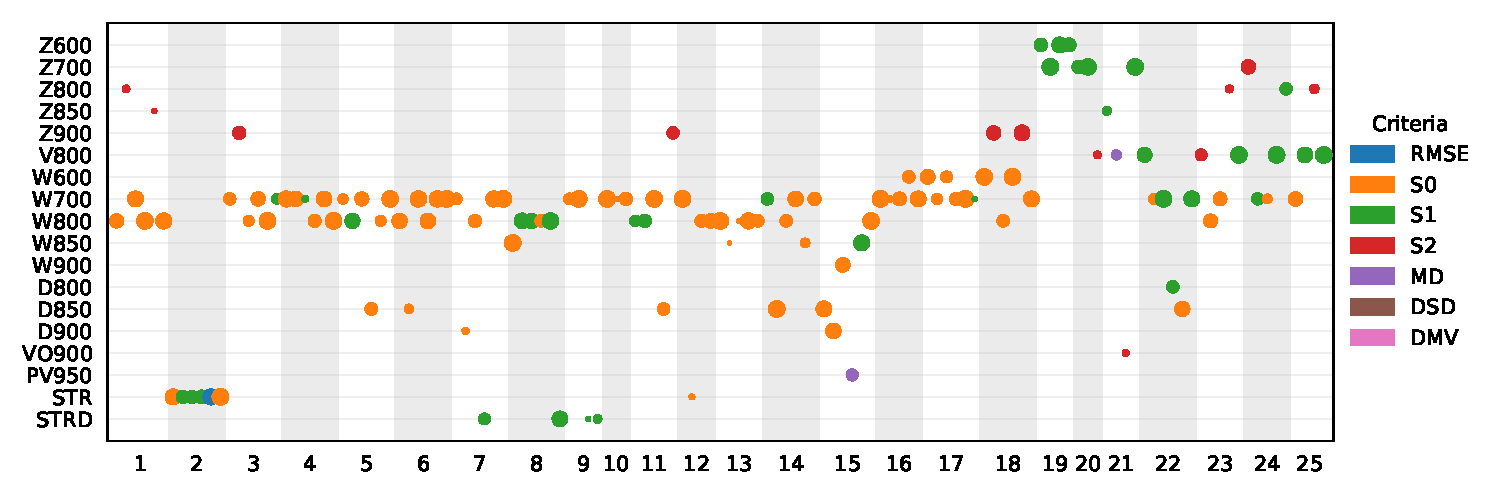
\includegraphics[width=170mm]{figures/single-variables-ERA-I.pdf}
	}
	\caption{Selected best variable for ERA-INT.}
	\label{fig_best_era_int}
\end{figure}

\begin{figure}[hbt]
	\noindent\makebox[\textwidth]{
		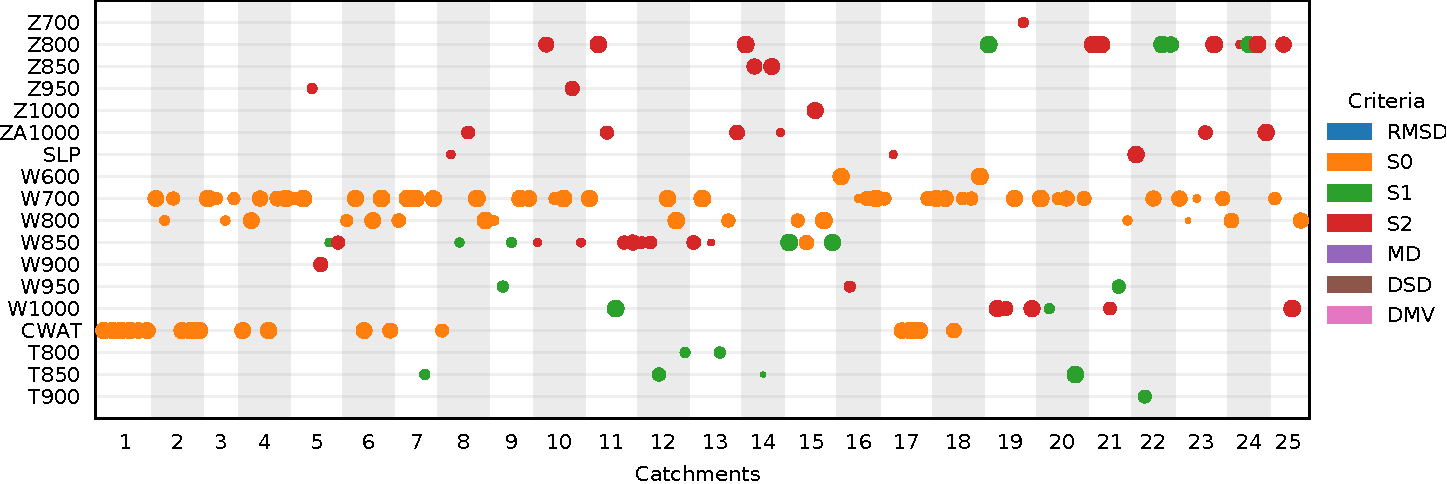
\includegraphics[width=170mm]{figures/single-variables-CFSR.pdf}
	}
	\caption{Selected best variable for CFSR.}
	\label{fig_best_cfsr}
\end{figure}

\begin{figure}[hbt]
	\noindent\makebox[\textwidth]{
		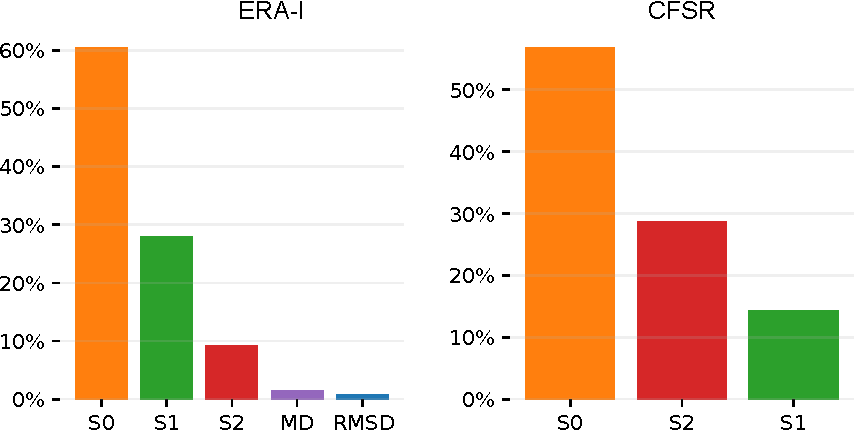
\includegraphics[width=90mm]{figures/criteria.pdf}
	}
	\caption{Selected best criteria.}
	\label{fig_criteria}
\end{figure}

\subsection{Assessing AM Structures}
\label{structures}

\todo[inline]{matrix of n levels of analogy x n predictors}
\todo[inline]{assess gains vs overfitting}
\todo[inline]{assess most performing GAs operators}



The results also depicted significant differences between the mutation operators (Sect. \ref{gas}). The chromosome of adaptive search radius (option \#1) resulted in the best performing parameters sets 76.3\% of the time for the calibration period, and 62.5\% of the time for the validation period (Fig. \ref{fig_mutation_operators_perfs}).  The second best is the non-uniform mutation with a mutation probability ($p_{mut}$) of 0.1 (option \#4) with a success rate of 11.3\% for the calibration period and 21.3\% for the validation period. However, the same operator with a  mutation probability ($p_{mut}$) of 0.2 (option \#5; $G_{m,r}$=100) is the worst performing option, with a success rate of 1.3\% for the calibration period and 2.5\% for the validation period. This quite well illustrate the difficulty of tuning such operators and the risk of a badly-parametrized mutation operator and the benefit of a auto-adaptive operator such as the chromosome of adaptive search radius that has no controlling parameter. Moreover, this operator was also usually performing better for more complex structures of the AM.




\begin{figure}[hbt]
	\noindent\makebox[\textwidth]{
		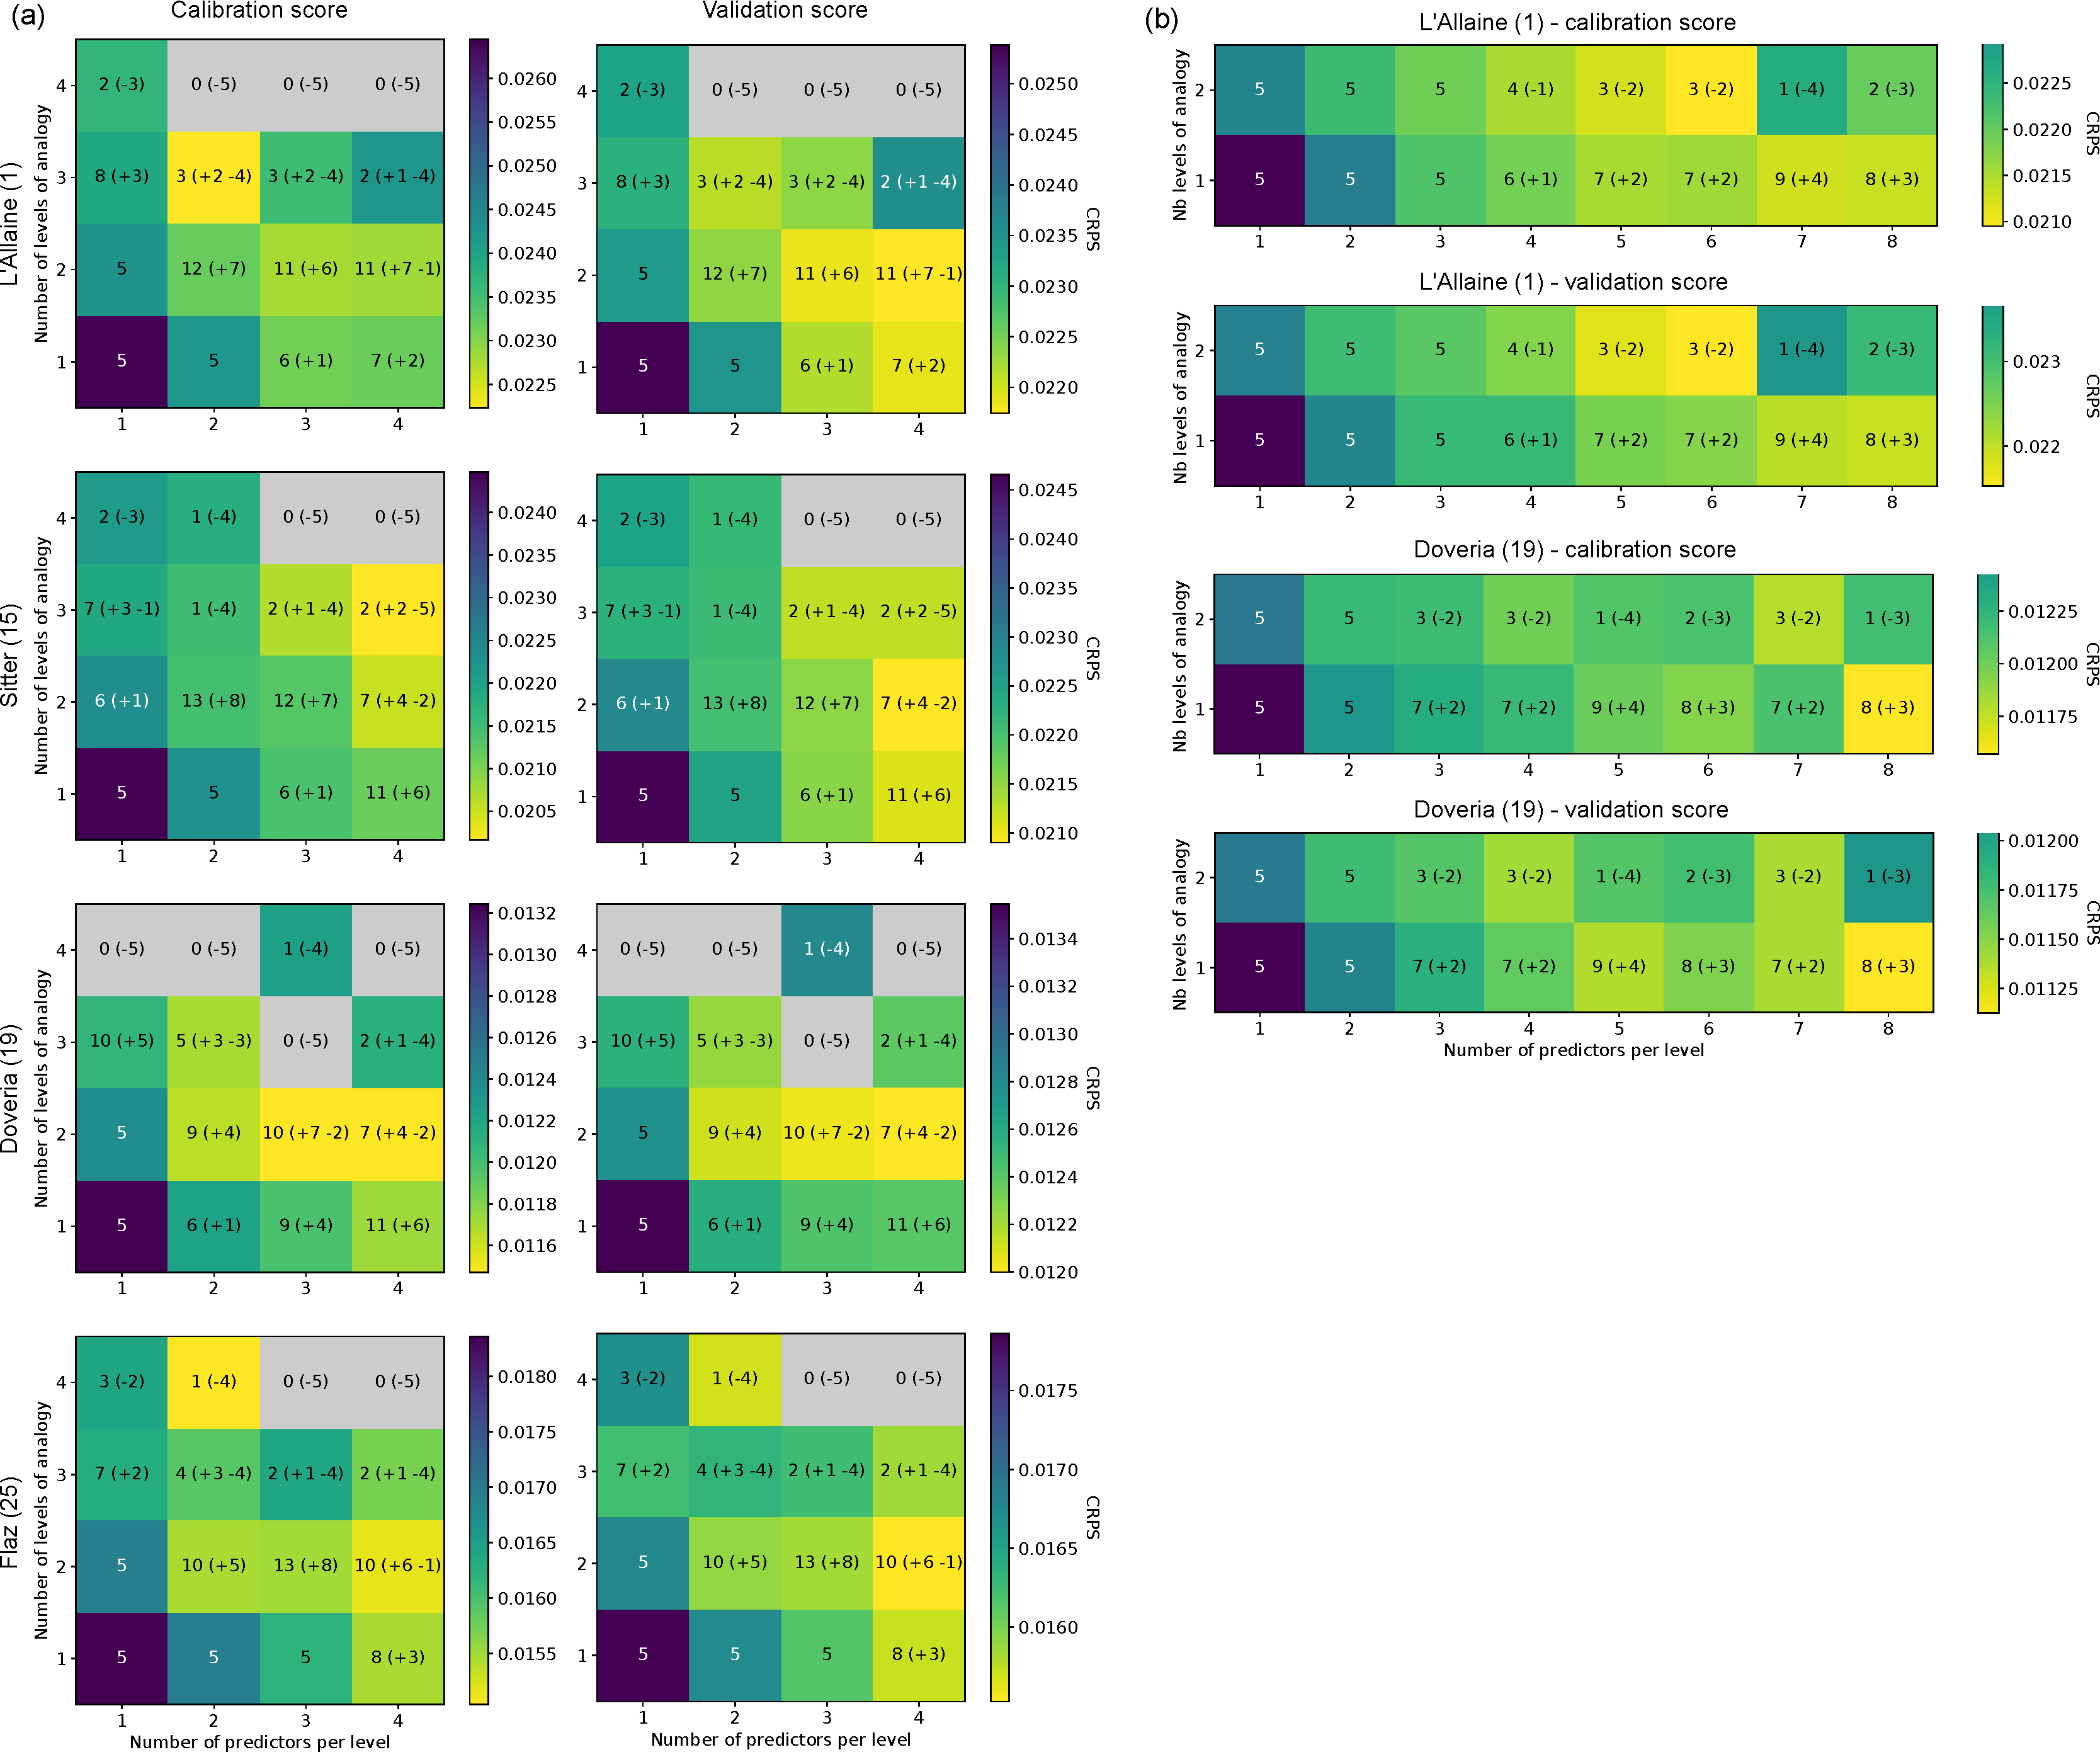
\includegraphics[width=180mm]{figures/ams-structures.pdf}
	}
	\caption{Selected best variable for CFSR.}
	\label{fig_structures}
\end{figure}


\subsection{Best Variables Combination}
\label{best_multi}

* weight: iteration="0.01"
* only the chromosome of adaptive search radius


\todo[inline]{optimize with relevant structure for all catchments. remove criteria and variables that were not selected before ? Adjust max domain ?}
\todo[inline]{try to build 1 common AM for all catchments (same predictors, different weights)}
\todo[inline]{compare skill with existing AMs}
\todo[inline]{distribution of the weights?}
\todo[inline]{distribution of the hours?}

Issue with radiation data: \cite{Boilley2015}.

\begin{figure}[hbt]
	\noindent\makebox[\textwidth]{
		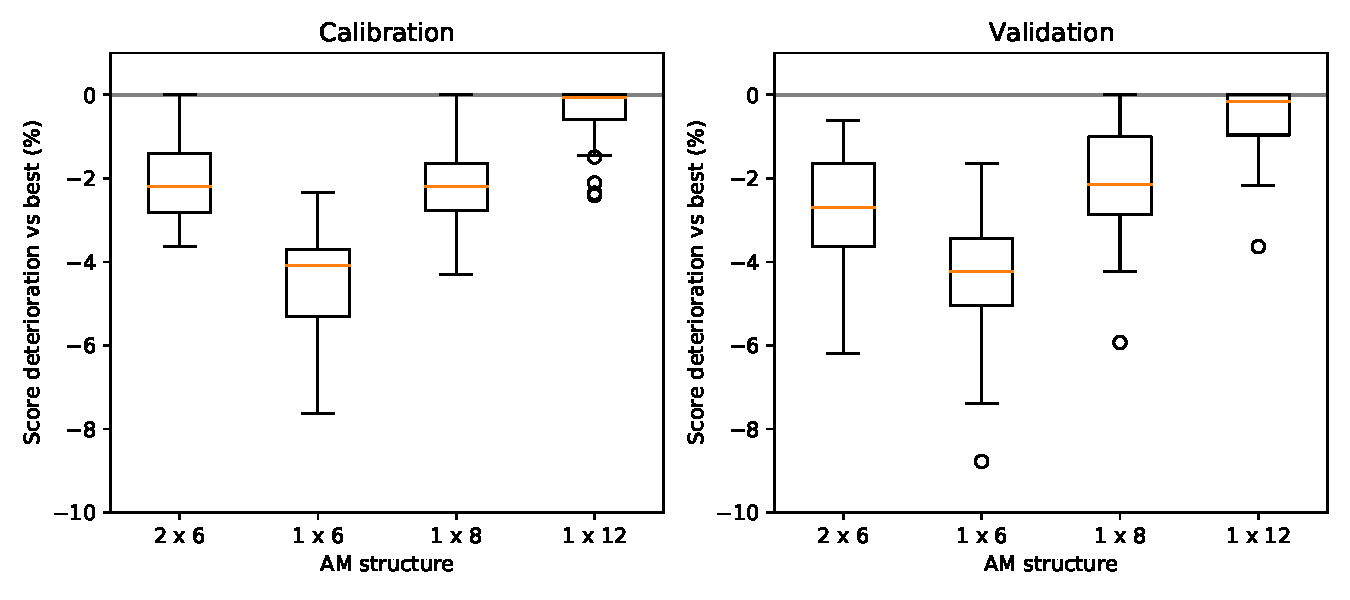
\includegraphics[width=160mm]{figures/multiple-variables-structures.pdf}
	}
	\caption{Assessed AM structures.}
	\label{fig_multiple_variables_structures}
\end{figure}

\begin{figure}[hbt]
	\noindent\makebox[\textwidth]{
		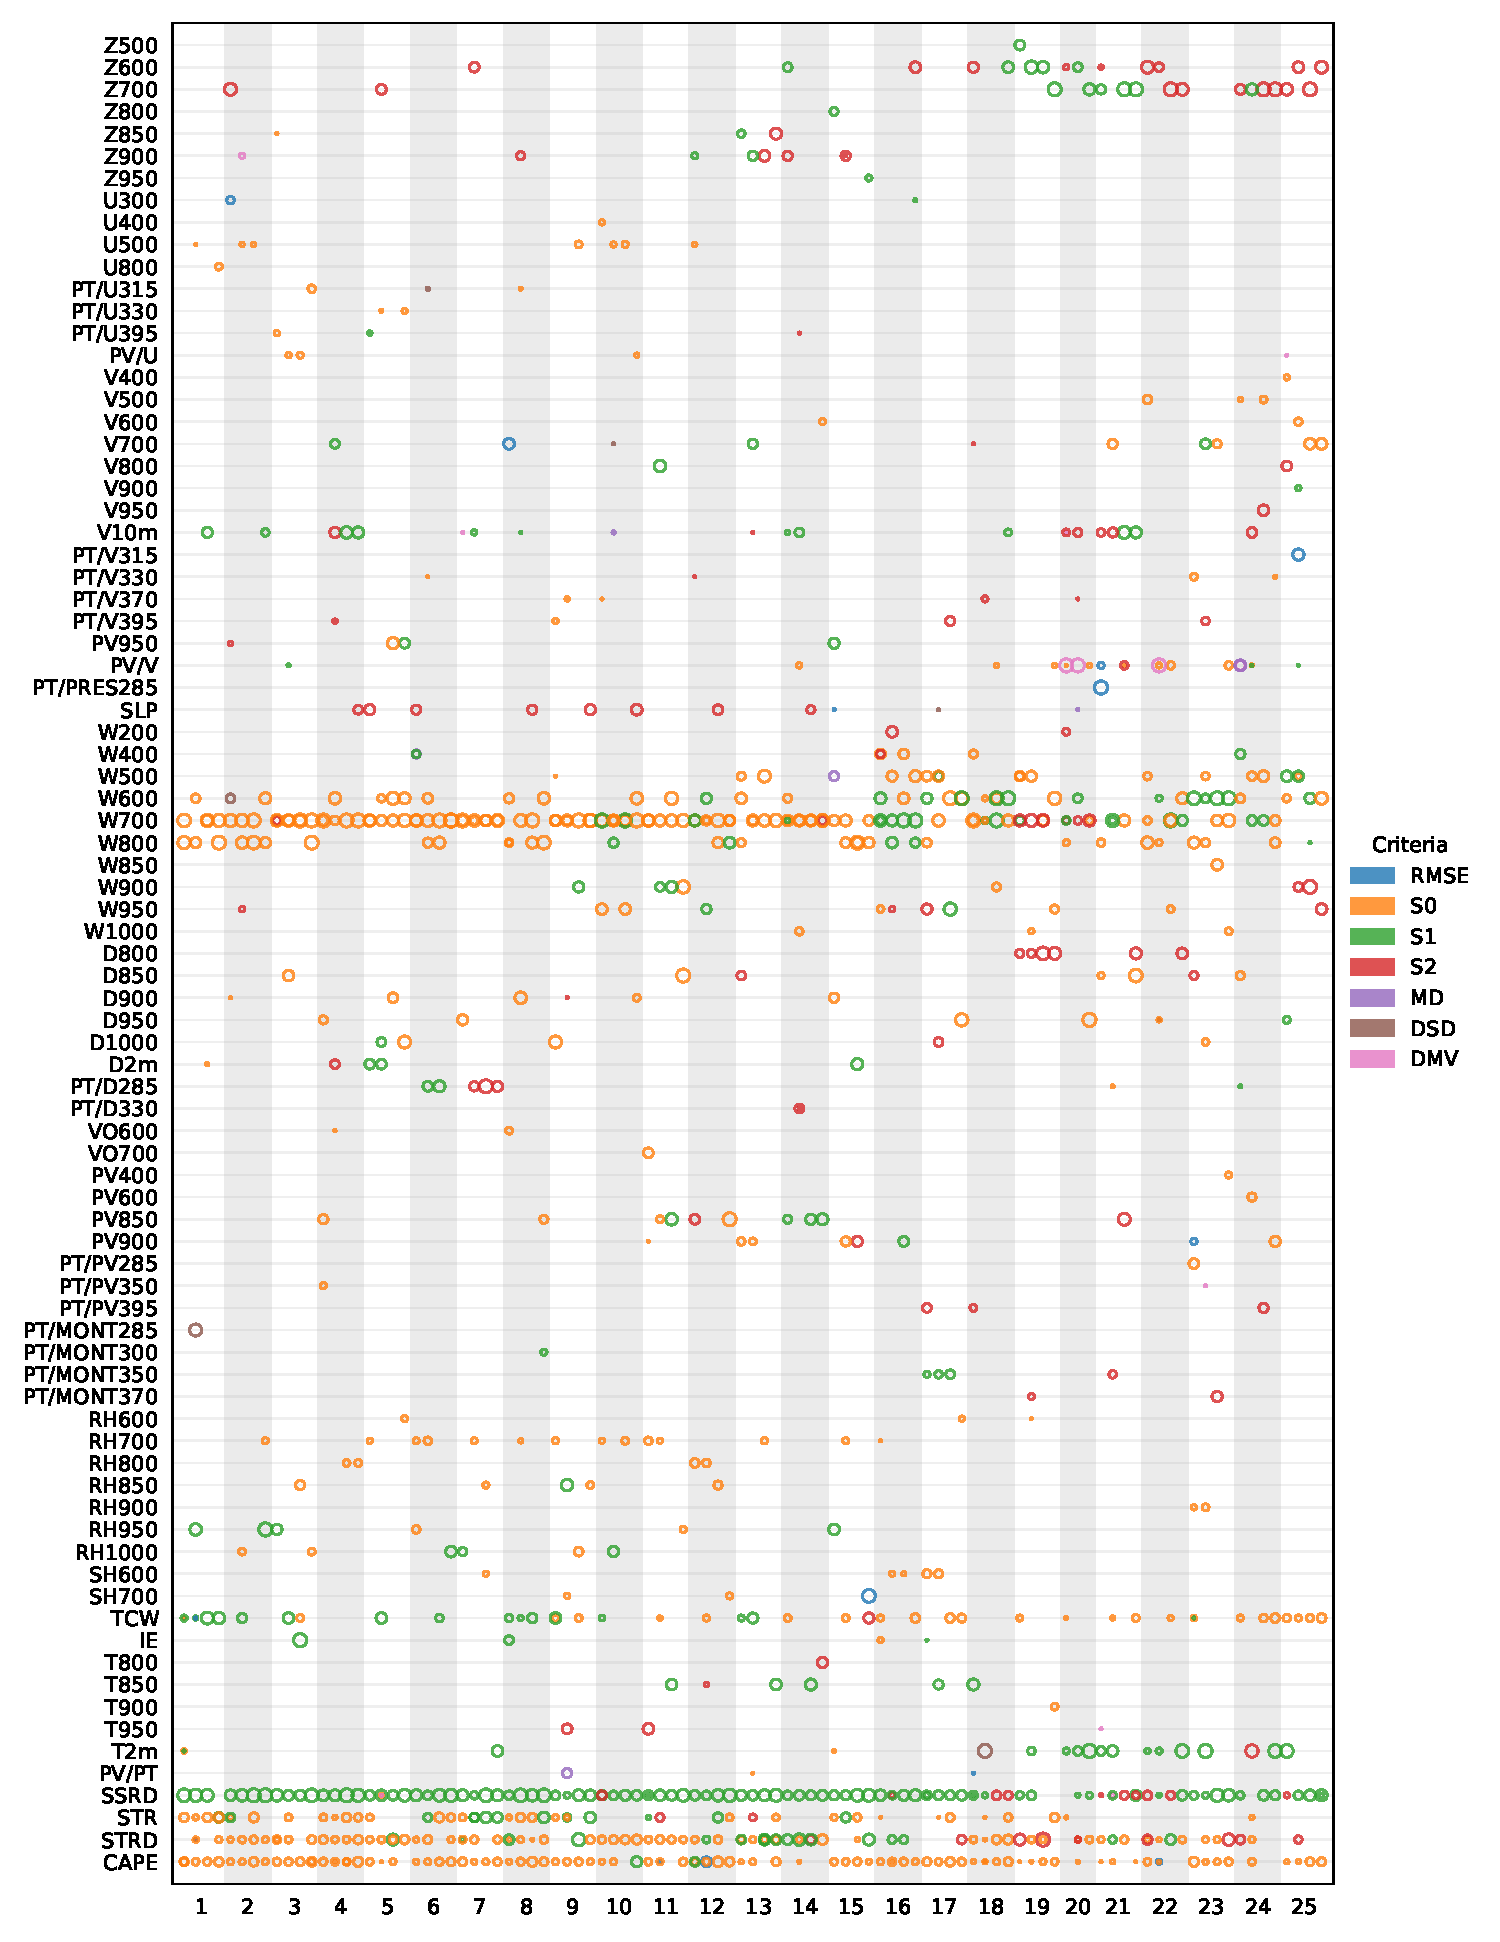
\includegraphics[width=180mm]{figures/multiple-variables.pdf}
	}
	\caption{Selected 8/12 variables for the different catchments.}
	\label{fig_multiple_variables}
\end{figure}

\begin{figure}[hbt]
	\noindent\makebox[\textwidth]{
		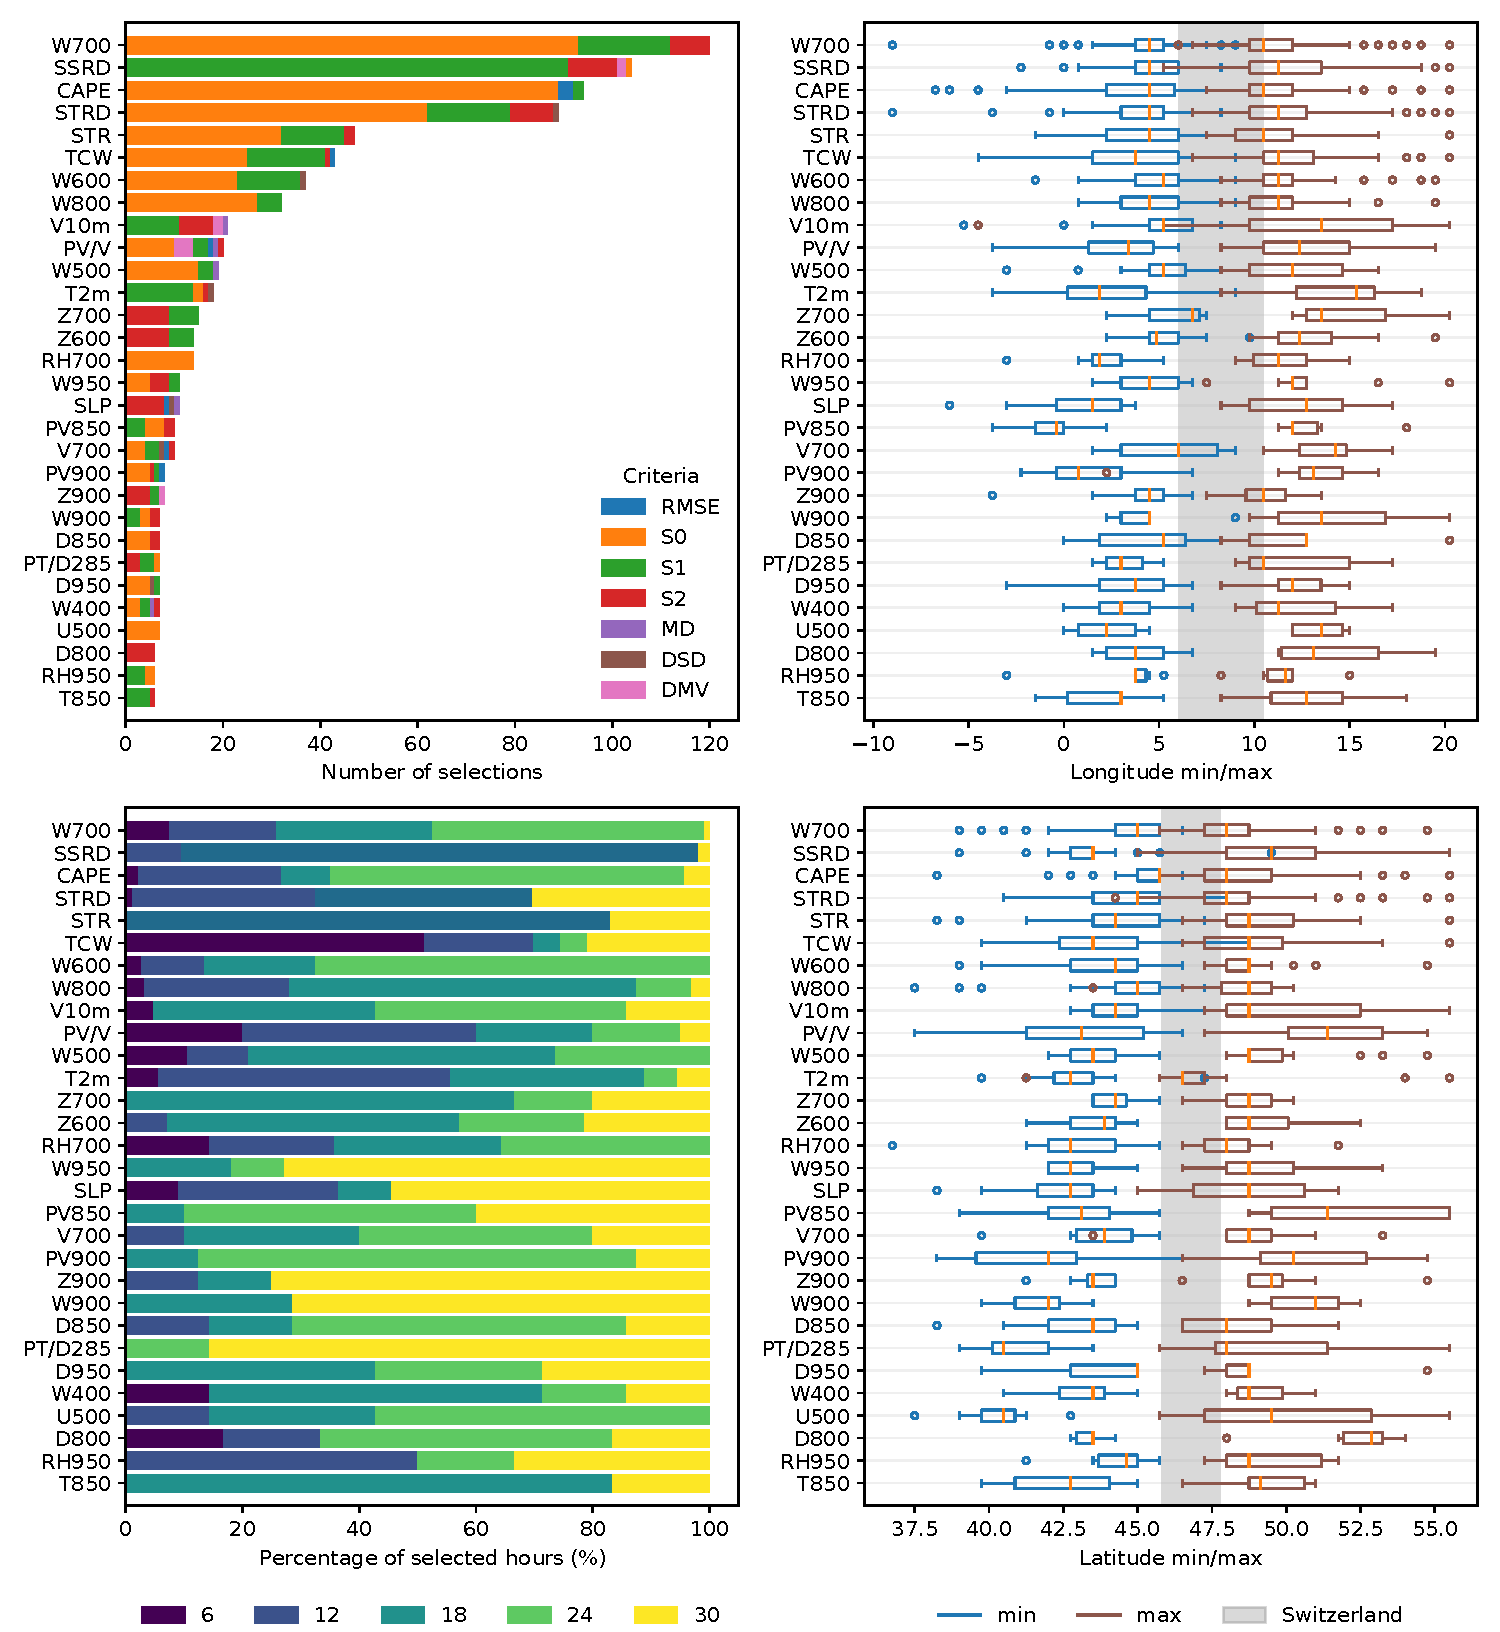
\includegraphics[width=160mm]{figures/multiple-variables-summary.pdf}
	}
	\caption{Most selected variables and their weighting.}
	\label{fig_variables_weights}
\end{figure}


\section{Discussion}
\label{discussion}

\subsection{Meteorological processes behind the selected variables}


\subsection{Why does S0 perform so well?}


\subsection{Computational burden}

* work on a smaller calibration period


\section{Conclusions}
\label{conclusions}




%% Enter Figures and Tables near as possible to where they are first mentioned:
%
% DO NOT USE \psfrag or \subfigure commands.
%
% Figure captions go below the figure.
% Table titles go above tables;  other caption information
%  should be placed in last line of the table, using
% \multicolumn2l{$^a$ This is a table note.}
%
%----------------
% EXAMPLE FIGURES
%
% \begin{figure}
% \includegraphics{example.png}
% \caption{caption}
% \end{figure}
%
% Giving latex a width will help it to scale the figure properly. A simple trick is to use \textwidth. Try this if large figures run off the side of the page.
% \begin{figure}
% \noindent\includegraphics[width=\textwidth]{anothersample.png}
%\caption{caption}
%\label{pngfiguresample}
%\end{figure}
%
%
% If you get an error about an unknown bounding box, try specifying the width and height of the figure with the natwidth and natheight options. This is common when trying to add a PDF figure without pdflatex.
% \begin{figure}
% \noindent\includegraphics[natwidth=800px,natheight=600px]{samplefigure.pdf}
%\caption{caption}
%\label{pdffiguresample}
%\end{figure}
%
%
% PDFLatex does not seem to be able to process EPS figures. You may want to try the epstopdf package.
%

%
% ---------------
% EXAMPLE TABLE
%
% \begin{table}
% \caption{Time of the Transition Between Phase 1 and Phase 2$^{a}$}
% \centering
% \begin{tabular}{l c}
% \hline
%  Run  & Time (min)  \\
% \hline
%   $l1$  & 260   \\
%   $l2$  & 300   \\
%   $l3$  & 340   \\
%   $h1$  & 270   \\
%   $h2$  & 250   \\
%   $h3$  & 380   \\
%   $r1$  & 370   \\
%   $r2$  & 390   \\
% \hline
% \multicolumn{2}{l}{$^{a}$Footnote text here.}
% \end{tabular}
% \end{table}

%% SIDEWAYS FIGURE and TABLE
% AGU prefers the use of {sidewaystable} over {landscapetable} as it causes fewer problems.
%
% \begin{sidewaysfigure}
% \includegraphics[width=20pc]{figsamp}
% \caption{caption here}
% \label{newfig}
% \end{sidewaysfigure}
%
%  \begin{sidewaystable}
%  \caption{Caption here}
% \label{tab:signif_gap_clos}
%  \begin{tabular}{ccc}
% one&two&three\\
% four&five&six
%  \end{tabular}
%  \end{sidewaystable}

%% If using numbered lines, please surround equations with \begin{linenomath*}...\end{linenomath*}
%\begin{linenomath*}
%\begin{equation}
%y|{f} \sim g(m, \sigma),
%\end{equation}
%\end{linenomath*}

%%% End of body of article

%%%%%%%%%%%%%%%%%%%%%%%%%%%%%%%%
%% Optional Appendix goes here
%
% The \appendix command resets counters and redefines section heads
%

\FloatBarrier

\appendix

\section{Benchmarks of the GPU implementation}

\begin{figure}
	\noindent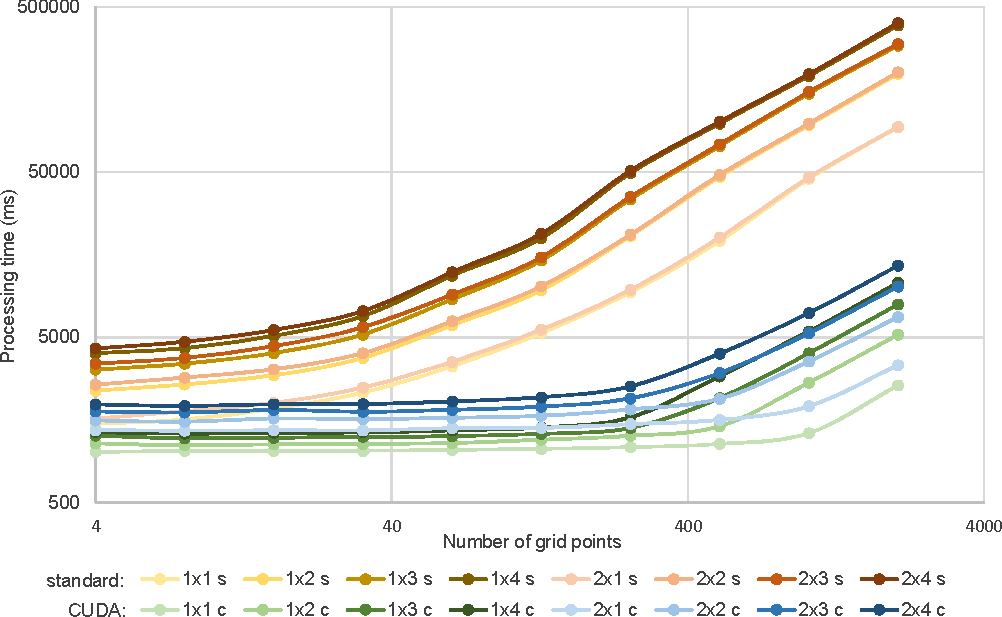
\includegraphics[width=130mm]{figures/cuda-timing.pdf}
	\caption{Processing time for the extraction of analogs over 32 years using the S1 criteria for different grid sizes and various structures of AMs. The structures are represented by a LxP code, L being the number of levels of analogy, and P being the number of predictors per level. Time is given for the use of (s) standard CPUs and (c) CUDA on GPUs. Note the logarithmic axes.}
	\label{cuda}
\end{figure}

The Google benchmark library was used to assess the processing time of different structures of the AM -- a single or two levels of analogy and up to four predictors per level -- along with various grid sizes. Figure \ref{cuda} shows the results for the analogy criterion S1, with gradients being pre-processed using CPUs only (counted in the total time). The other analogy criteria showed similar results. The task consisted in extracting analogs for 32 years by using the other 31 years as archive for candidate situations, within a 120~days temporal window. This makes a total of $43.5\cdot10^6$ field comparisons per predictor of the first level of analogy.

The experiment was conducted on the cluster of the University of Bern, using the same node for the whole benchmark, processing on a single NVIDIA GeForce RTX 2080 graphics card. The processing on the CPU -- using the linear algebra library Eigen 3 \cite{Guennebaud2010} -- was done on a single thread. Although AtmoSwing can parallelize the calculation of the analogy criteria on multiple CPU threads, it is using a single thread for this task when optimizing with GAs because it parallelizes the evaluation of the different individuals on multiple threads. Now, with the use of GPUs, it still assesses the individuals on multiple CPU threads, each of them being able to exploit a different GPU device for the calculation of the analogy criteria. It is thus parallelizing both on CPUs and GPUs.

The benchmark (Fig. \ref{cuda}) shows that the calculations on the GPU are systematically faster than those on the CPU, and this difference increases with the number of grid points. The calculations on the GPU were 13 times faster in average, and up to a maximum of 38 times faster (5.2~sec instead of 3.3~min) when using 2048 points. Model outputs and reanalyses show an increase in spatial resolution and thus this will become increasingly important. When using CPU only, the addition of a predictor in the first level of analogy has a much higher impact on time than the addition of a second level of analogy. This is explained by the fact that it needs to process the analogy criteria for the whole archive for each predictor of the first level of analogy, while the second level has only few candidate situations to assess.

%TODO: add comparison with multiple CPUs


\section{Performance of the mutation operators}


Success percentages:
calib: [76.25  7.5  11.25 11.25  1.25]
valid : [62.5   8.75 10.   21.25  2.5 ]

\begin{figure}
	\noindent\makebox[\textwidth]{
		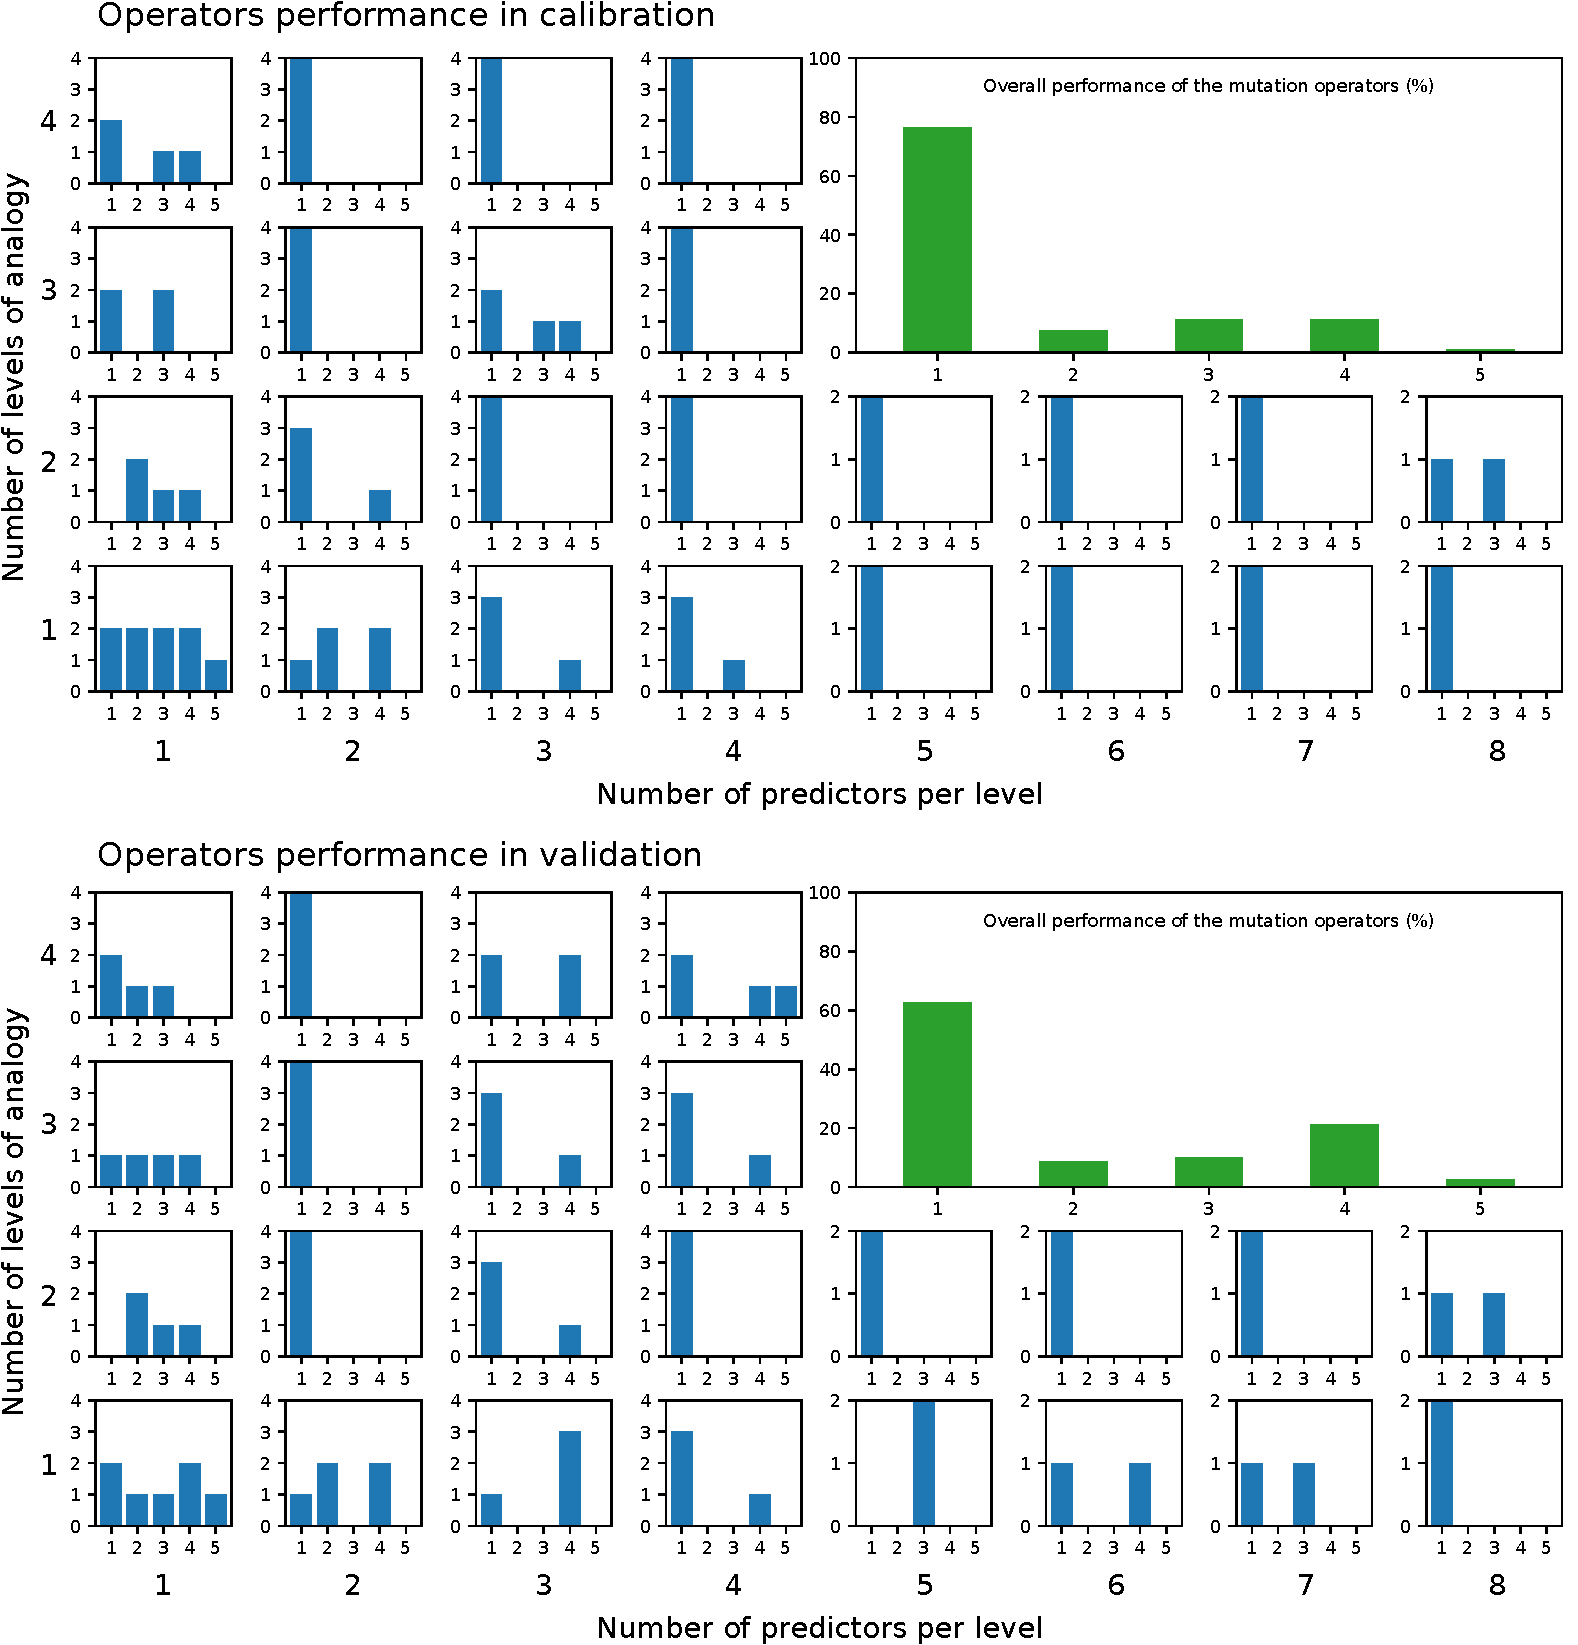
\includegraphics[width=170mm]{figures/gas-configs-ams-structures.pdf}
	}
	\caption{...}
	\label{fig_mutation_operators_perfs}
\end{figure}



%%%%%%%%%%%%%%%%%%%%%%%%%%%%%%%%%%%%%%%%%%%%%%%%%%%%%%%%%%%%%%%%
%
% Optional Glossary, Notation or Acronym section goes here:
%
%%%%%%%%%%%%%%
% Glossary is only allowed in Reviews of Geophysics
%  \begin{glossary}
%  \term{Term}
%   Term Definition here
%  \term{Term}
%   Term Definition here
%  \term{Term}
%   Term Definition here
%  \end{glossary}

%
%%%%%%%%%%%%%%
% Acronyms
%   \begin{acronyms}
%   \acro{Acronym}
%   Definition here
%   \acro{EMOS}
%   Ensemble model output statistics
%   \acro{ECMWF}
%   Centre for Medium-Range Weather Forecasts
%   \end{acronyms}

%
%%%%%%%%%%%%%%
% Notation
%   \begin{notation}
%   \notation{$a+b$} Notation Definition here
%   \notation{$e=mc^2$}
%   Equation in German-born physicist Albert Einstein's theory of special
%  relativity that showed that the increased relativistic mass ($m$) of a
%  body comes from the energy of motion of the body—that is, its kinetic
%  energy ($E$)—divided by the speed of light squared ($c^2$).
%   \end{notation}

\FloatBarrier

\acknowledgments
Precipitation time series were provided by MeteoSwiss. The catchment extents were provided by the Hydrological Atlas of Switzerland (hydrologicalatlas.ch). The ERA-Interim reanalysis was obtained from the ECMWF Data Server at http://apps.ecmwf.int/datasets. The Climate Forecast System Reanalysis (CFSR) was obtained from the Computational \& Information Systems Lab (CISL) Research Data Archive (http://rda.ucar.edu/). The CFSR project is carried out by the Environmental Modeling Center (EMC), National Centers for Environmental Prediction (NCEP). Calculations were performed on UBELIX (http://www.id.unibe.ch/hpc), the HPC cluster at the University of Bern. 


%% ------------------------------------------------------------------------ %%
%% References and Citations

\bibliography{references}


%Reference citation instructions and examples:
%
% Please use ONLY \cite and \citeA for reference citations.
% \cite for parenthetical references
% ...as shown in recent studies (Simpson et al., 2019)
% \citeA for in-text citations
% ...Simpson et al. (2019) have shown...
%
%
%...as shown by \citeA{jskilby}.
%...as shown by \citeA{lewin76}, \citeA{carson86}, \citeA{bartoldy02}, and \citeA{rinaldi03}.
%...has been shown \cite{jskilbye}.
%...has been shown \cite{lewin76,carson86,bartoldy02,rinaldi03}.
%... \cite <i.e.>[]{lewin76,carson86,bartoldy02,rinaldi03}.
%...has been shown by \cite <e.g.,>[and others]{lewin76}.
%
% apacite uses < > for prenotes and [ ] for postnotes
% DO NOT use other cite commands (e.g., \citet, \citep, \citeyear, \nocite, \citealp, etc.).
%



\end{document}



More Information and Advice:

%% ------------------------------------------------------------------------ %%
%
%  SECTION HEADS
%
%% ------------------------------------------------------------------------ %%

% Capitalize the first letter of each word (except for
% prepositions, conjunctions, and articles that are
% three or fewer letters).

% AGU follows standard outline style; therefore, there cannot be a section 1 without
% a section 2, or a section 2.3.1 without a section 2.3.2.
% Please make sure your section numbers are balanced.
% ---------------
% Level 1 head
%
% Use the \section{} command to identify level 1 heads;
% type the appropriate head wording between the curly
% brackets, as shown below.
%
%An example:
%\section{Level 1 Head: Introduction}
%
% ---------------
% Level 2 head
%
% Use the \subsection{} command to identify level 2 heads.
%An example:
%\subsection{Level 2 Head}
%
% ---------------
% Level 3 head
%
% Use the \subsubsection{} command to identify level 3 heads
%An example:
%\subsubsection{Level 3 Head}
%
%---------------
% Level 4 head
%
% Use the \subsubsubsection{} command to identify level 3 heads
% An example:
%\subsubsubsection{Level 4 Head} An example.
%
%% ------------------------------------------------------------------------ %%
%
%  IN-TEXT LISTS
%
%% ------------------------------------------------------------------------ %%
%
% Do not use bulleted lists; enumerated lists are okay.
% \begin{enumerate}
% \item
% \item
% \item
% \end{enumerate}
%
%% ------------------------------------------------------------------------ %%
%
%  EQUATIONS
%
%% ------------------------------------------------------------------------ %%

% Single-line equations are centered.
% Equation arrays will appear left-aligned.

Math coded inside display math mode \[ ...\]
 will not be numbered, e.g.,:
 \[ x^2=y^2 + z^2\]

 Math coded inside \begin{equation} and \end{equation} will
 be automatically numbered, e.g.,:
 \begin{equation}
 x^2=y^2 + z^2
 \end{equation}


% To create multiline equations, use the
% \begin{eqnarray} and \end{eqnarray} environment
% as demonstrated below.
\begin{eqnarray}
  x_{1} & = & (x - x_{0}) \cos \Theta \nonumber \\
        && + (y - y_{0}) \sin \Theta  \nonumber \\
  y_{1} & = & -(x - x_{0}) \sin \Theta \nonumber \\
        && + (y - y_{0}) \cos \Theta.
\end{eqnarray}

%If you don't want an equation number, use the star form:
%\begin{eqnarray*}...\end{eqnarray*}

% Break each line at a sign of operation
% (+, -, etc.) if possible, with the sign of operation
% on the new line.

% Indent second and subsequent lines to align with
% the first character following the equal sign on the
% first line.

% Use an \hspace{} command to insert horizontal space
% into your equation if necessary. Place an appropriate
% unit of measure between the curly braces, e.g.
% \hspace{1in}; you may have to experiment to achieve
% the correct amount of space.


%% ------------------------------------------------------------------------ %%
%
%  EQUATION NUMBERING: COUNTER
%
%% ------------------------------------------------------------------------ %%

% You may change equation numbering by resetting
% the equation counter or by explicitly numbering
% an equation.

% To explicitly number an equation, type \eqnum{}
% (with the desired number between the brackets)
% after the \begin{equation} or \begin{eqnarray}
% command.  The \eqnum{} command will affect only
% the equation it appears with; LaTeX will number
% any equations appearing later in the manuscript
% according to the equation counter.
%

% If you have a multiline equation that needs only
% one equation number, use a \nonumber command in
% front of the double backslashes (\\) as shown in
% the multiline equation above.

% If you are using line numbers, remember to surround
% equations with \begin{linenomath*}...\end{linenomath*}

%  To add line numbers to lines in equations:
%  \begin{linenomath*}
%  \begin{equation}
%  \end{equation}
%  \end{linenomath*}



